% ****** Start of file aipsamp.tex ******
%
%   This file is part of the AIP files in the AIP distribution for REVTeX 4.
%   Version 4.1 of REVTeX, October 2009
%
%   Copyright (c) 2009 American Institute of Physics.
%
%   See the AIP README file for restrictions and more information.
%
% TeX'ing this file requires that you have AMS-LaTeX 2.0 installed
% as well as the rest of the prerequisites for REVTeX 4.1
% 
% It also requires running BibTeX. The commands are as follows:
%
%  1)  latex  aipsamp
%  2)  bibtex aipsamp
%  3)  latex  aipsamp
%  4)  latex  aipsamp
%
% Use this file as a source of example code for your aip document.
% Use the file aiptemplate.tex as a template for your document.
\documentclass[%
 aip,
% jmp,
% bmf,
% sd,
% rsi,
 amsmath,amssymb,
preprint,%
% reprint,%
%author-year,%
%author-numerical,%
% Conference Proceedings
]{revtex4-1}

\usepackage{graphicx}% Include figure files
\usepackage{dcolumn}% Align table columns on decimal point
\usepackage{bm}% bold math
%\usepackage[mathlines]{lineno}% Enable numbering of text and display math
%\linenumbers\relax % Commence numbering lines

\usepackage[utf8]{inputenc}
\usepackage[T1]{fontenc}
\usepackage{mathptmx}
\usepackage{etoolbox}
\graphicspath{{images/}}
%% Apr 2021: AIP requests that the corresponding  
%% email to be moved after the affiliations
\makeatletter
\def\@email#1#2{%
 \endgroup
 \patchcmd{\titleblock@produce}
  {\frontmatter@RRAPformat}
  {\frontmatter@RRAPformat{\produce@RRAP{*#1\href{mailto:#2}{#2}}}\frontmatter@RRAPformat}
  {}{}
}%
\usepackage{xcolor}
\makeatother
\begin{document}

\preprint{AIP/123-QED}

%\title[Aerothermal for hypersonic reentry vehicles]{Aerothermal conjugate heating transfer estimation for hypersonic reentry vehicles}
\title[Aerothermal assessment of reentry vehicles]{A predictive framework for aerothermal assessment of hypersonic reentry vehicles}
% Force line breaks with \\
\author{Jeswin Joseph}

\affiliation{ 
Department of Mechanical and Mechatronics Engineering, University of Waterloo, 200 University Ave. W., Waterloo, Ontario, Canada
}%


\author{Ryan Whitside}

\author{Bryan Godbolt}

\affiliation{%
Unmanned Vehicle Applied Dynamics (UVAD), Alberta, Canada
}%

\author{Jean-Pierre Hickey}

\affiliation{ 
Department of Mechanical and Mechatronics Engineering, University of Waterloo, 200 University Ave. W., Waterloo, Ontario, Canada
}%

\date{\today}% It is always \today, today,
             %  but any date may be explicitly specified

%\setauthorlist{Jeswin Joseph, Jean-Pierre Hickey}\setauthoraffiliation{  University of Waterloo, 200 University Ave. W., Waterloo, Ontario}\setauthorcountry{CANADA}

%\setauthorlist{Ryan Whitside, Bryan Godbolt}
%\setauthoraffiliation{Unmanned Vehicle Applied Dynamics (UVAD), 1500 South Highway Dr SE 1, Redcliff, Alberta }
%\setauthorcountry{CANADA}

\begin{abstract}
The identification and characterization of the maximum aerothermal load drives the thermal management and thermal protection system for hypersonic vehicle design.  Vehicle design, reentry or mission profiles, and attitude control can impart important changes to thermal loading. The accurate characterization of the thermal load represents a time-integrated, multi-scale problem with strong multi-physics coupling.  The present work proposes a multi-fidelity optimization framework to assist in the design considerations for high-speed reentry capsules or vehicles. Using a low-fidelity modeling approach, we propose the use of models for reentry trajectory simulation, entropic shock-heating, radiative exchanges, conjugate heat transfer with considerations for internal heat generation and thermal protection systems. These effects are integrated with unsteady time history trajectory estimation within the open-source framework Stanford University Aerospace Vehicle Environment (SUAVE), which enable vehicle design and trajectory optimization. Once identified, the local peak thermal load condition can be studied using high-fidelity numerical modeling under these time-varying conditions.
\end{abstract}

\maketitle


\section{ Introduction}
Hypersonic flight is at the technological frontier in the aerospace sector with applications in high-speed global transportation, defense, and atmospheric reentry. Analysis of several critical subcomponents and subsystems, such as structural, thermal mananagement systems, avionics, trajectory, and propulsion plays a vital role during the design phase of a hypersonic vehicle \citep{sziroczak_review_2016}; thermal management systems are of specific interest herein. The thermal management systems are designed around the characterization of the peak and the integrated aerothermal loading on the vehicle.  Thus, the aerothermal heat load estimation and heat transfer characterization greatly influence the design, weight, complexity, and reliability of the vehicle \citep{schmisseur_hypersonics_2015,yang_heat_2021}.

The aerothermal heat loads are time-varying and strongly influenced by the flow physics near the vehicle surface \citep{anderson_hypersonic_2019}. When a hypersonic vehicle travels through the atmosphere, the deflection of the air is achieved through a series of expansion and shock waves. 
Across a hypersonic shock, the thermodynamic properties such as pressure, density, temperature, and entropy increase drastically. Depending on the bluntness of the leading edge, the enhancement of entropy gradients close to the nose region can result in very large heat flux. The presence of shocks, and especially shock boundary layer or shock-shock interactions, act to amplify the turbulence intensity and further increase post-shock temperature and wall heat flux.  Thus, the characterization of the post-shock state is a key component to aerothermal prediction, which in turn depends on the kinematic trajectory and atmospheric conditions during the mission.

In addition to shock-induced heating, high-speed flow over solid walls generates a boundary layer that slows the fluid while increasing its temperature; this can occur in addition to the entropy layer caused by the leading edge shock. The state of the boundary layer can greatly influence the heat transfer to the vehicle.  Higher gradients in the turbulent boundary layer lead to stronger near-wall temperature gradients and, consequently, to higher aerothermal heat loads over the vehicle walls. However, the amount of heat transferred to the vehicle depends on the wall temperature, which is also strongly coupled to the integrated flight trajectory, convective and radiative losses, active or passive cooling, conductive heat transfer within the vehicle as well as any internal heat sources such as propulsion systems. 

%\textcolor{red}{Need to discuss radiative, ablative, TPS etc here.}

Considering these strongly coupled multi-physics phenomena and conjugate heat transfer (CHT), predictive modeling of the peak and integrated aerothermal loading on hypersonic vehicles is a challenging design consideration.
Although higher-fidelity CFD methods can model these coupled phenomena, they are computationally expensive at predicting time-integrated aerothermal heat loads for an entire flight trajectory. In this regard, low-fidelity multi-physics models, in conjunction with higher-fidelity modeling approaches, are capable of providing a multi-fidelity predictive modeling framework of hypersonic thermal design. Thus, a multi-fidelity integrated framework is a vital tool to address the modeling challenges pertinent to time-integral aerothermal load prediction for hypersonic flight.


The accurate prediction of thermal loading in hypersonic vehicles represents a time-integrated problem; therefore, considering the history effects of these thermal loads is a necessary condition. The protection against the thermal loading constitutes one of the key opportunities to increase the re-entry corridor from a vehicle design and trajectory optimization perspective \cite{karl_sustainable_2024}. Low-fidelity hypersonic aerothermal models are simple numerical tools that represent heat transfer mechanisms at the interface of the vehicle surface and the surrounding atmosphere. Pioneering work in the prediction of aerodynamic and aerothermodynamic profiles in reference geometries was carried out by \citet{tauber_review_1989}. Panel methods were used for laminar flow, the reference temperature method for turbulent flow, and a linear blending function for the transitional regime. The approach led to development of non-linear mathematical models for flow physics around simple full-scale hypersonic vehicles. 

A predictive tool for aerothermal heating was developed by \citet{Quinn_2000} in 2000 called TPATH, which is capable of simulating transient surface heat flux and temperatures at hypersonic speeds using convective-heating methods and approximate heat conduction method, respectively. The model was used by \citet{Ko_Gong_Quinn_2007} to simulate the aerothermal performance of Apollo 9 mission.

\citet{Paxton_Villasenor_Gallagher_Chun_2020} used the Configuration-Based Aerodynamics (CBAERO) tool developed by Kinney in 2004 using panel method for hypersonic aerodynamics, along with high-fidelity CFD++ simulations, to compare the multi-fidelity predictions with aerothermal test results over the Hypersonic International Flight Research Experimentation (HIFiRE-5) body. They found that the model behaved well under standard conditions, but poorly predicted the boundary-layer transition.

Object Reentry Survival Analysis Tool (ORSAT) is a simulation program developed by \citet{Dobarco-Otero_Smith_Bledsoe_DeLaune_Rochelle_Johnson_2005} in 2005 to assess the risks associated with uncontrolled reentry of spacecraft and rocket bodies. The program uses Global Reference Atmospheric Model developed by NASA, cosine law for surface heat flux predictions and melting model for surface ablation. The program was used by \cite{Ostrom_Greene_Smith_Toledo-Burdett_Matney_Opiela_Marichalar_Bacon_Sanchez} to typical debris reentry conditions. They noted that further improvement is required to the model to handle aerodynamics, conduction and spatially varying heat flux distribution.



Debris Risk Assessment and Mitigation Analysis (DRAMA) tool developed by European Space Agency (ESA) (Fuentes et al in 2017 and Braun et al in 2020) is another debris management tool estimates aerothermodynamic coefficients for multiple primitive shapes representing spacecraft fragments during reentry. This object-oriented approach to predict aerothermodynamics using analytical formulations and pre-computed databases for simple geometrical shapes.

Heat flux estimation using Newtonian velocity gradient at stagnation point was used by Gonclaves et al in 2020 in association with predictive aerodynamic tool called Stanford University Aerospace Vehicle Environment (SUAVE). The model predicted the heat flux profile of Intermediate eXperimental Vehicle (IXV) under reentry conditions, however lacked the surface heat flux and temperature profile predictions.

\citet{Laureti_Karl_2022} developed a surrogate model in 2022 for predicting aerothermodynamic heating over Retro Propulsion-Assisted Launch Vehicles (RETALT) using representative CFD simulation database. Their simulation model included reactive atmosphere, plume exhaust interaction chemistry and heat flux predictions using scaling laws at non-critical flight conditions. The multi-fidelity tool is valuable to preliminary evaluation of aerothermal loads over retro-firing reentry vehicle and have scope for improvement in its turbulence modelling assumptions.

More recently in 2023, a multi-fidelity hypersonic aerothermal predictive tool was developed by \cite{Kirsch_Lance_Krueger_Freno_2023} called Sandia Parallel Aerodynamics and Reentry Code (SPARC) using Reynolds-Averaged Navier-Stokes (RANS) based CFD solver, momentum-energy integral technique and panel methods to achieve different fidelity levels for hypersonic reentry prediction. The model is validated against HIFiRE-1 experiments and simulation results showed significant deviation from heat flux data even for high-fidelity CFD results. Their low-fidelity panel methods were insufficient in predicting surface heat flux variations which was attributed to inaccuracies in distributed momentum thickness estimates.

Finally in 2024, \cite{morgado_multifidelity_2024} introduced the shock environment around re-entry debris to their multi-fidelity trans-atmospheric flight simulation tool called TITAN. They achieved this tool by applying Billig’s formulations9 to develop a physics-infused low-fidelity model, using panel methods and van Driest models for the boundary layer profile. Internal heat transfer in the low-fidelity framework is modeled as lumped parameters. The model was supported by SU2-NEMO in continuum regime applications and a Direct Simulation Monte Carlo (DSMC) solver in rarefied flow. They developed a physics-based automated switch between low- and high-fidelity tools and introduced local adaptive meshes around complex geometries to improve simulation accuracy.





ROM frameworks use CFD flow parameters and / or structural parameters to derive a surrogate model of aerothermal heat load \citep{crowell_reduced_2010}, which makes them computationally more expensive than low-fidelity models. A low-fidelity mathematical framework is structured using the flow field formulations from first principles and utilizes the near-wall behavior of flow parameters to derive the aerothermal surrogate model, which can predict vehicle aerodynamic parameters for a given mission. The model fidelity can be enhanced using CFD results, where parametric complexity (e.g. vehicle, trajectory, maneuver) exists, bringing about its multi-fidelity capabilities. Since low-fidelity models are nimble in predicting aerothermal heating with minimal intervention of high-fidelity tools, they are suitable for large-scale temporal and spatial aerothermal load predictions.  




All the low-fidelity tools mentioned above are developed to complement a multi-fidelity framework for predicting hypersonic aerothermodynamics. Among them, SUAVE stands out due to its diverse capabilities including multi-mode trajectory models, wide range of propulsion surrogates, multi-faceted aerodynamic models (performance, stability and noise estimates), component-level geometry development, high-fidelity switching and most importantly, nimble framework to optimize any of these model parameters. However, the present SUAVE framework lacks predictive aerothermal capabilities for hypersonic flight. In the present work, a detailed aerothermal module is developed and augmented to the SUAVE framework, making it an attractive tool in quick identification and low-fidelity estimation of critical mission points within a hypersonic flight trajectory.


The present work introduces a multi-fidelity framework with optimization capabilities, that can be used to estimate the peak and integrated thermal loading during a hypersonic mission or reentry profile. This framework is built within the SUAVE, which is a powerful open-source multi-fidelity tool, scripted in Python language, in-built with formulations for detailed geometry creation, multi-regime flight aerodynamics, propulsion systems, segmented mission trajectory design, and parametric optimization \citep{lukaczyk_suave_2015}. Within SUAVE's framework, these formulations directly provide low-fidelity predictions for flight performance parameters such as aerodynamic forces, propulsor performance, and overall mission profile. Flight profiles outside the bounds of low-fidelity predictions can be complemented with high-fidelity aerodynamic data in SUAVE, which extends its capabilities beyond traditional geometries \citep{macdonald_suave_2017}. Adding multi-fidelity parametric optimization capabilities \citep{macdonald_suave_2017-1}, SUAVE is an attractive tool for hypersonic vehicle design, analysis, and optimization. In the present study, SUAVE is augmented with low-fidelity aerothermal formulations for aerothermodynamic predictions of hypersonic ground take-off and space reentry missions, enabling optimization for thermal loads of both trajectory and geometry.

A description of the low-fidelity models integrated into SUAVE to enable these aerothermodynamic predictions is detailed in the next section. This is followed by a description of validation cases for the predictive framework against experimental and analytical reentry data. These include the stagnation point heat transfer validation results for the Intermediate eXperimental Vehicle (IXV), surface heat flux distributions behind the bow shock of test specimen of Orion crew exploration vehicle, and surface temperature estimation through the nonablative thermal protection system of the Apollo crew capsule for a generic reentry profile. 


\section{Methodology}
A lower order optimization framework for aerothermal heating with CHT must rely on a set of modeling assumptions to correctly reproduce the physics. The primary challenge in multi-fidelity frameworks lies in correctly aligning the computational tractability of the model with the requisite level of simplification and fidelity. The objective of the present framework is to develop a nimble, low-fidelity tool within SUAVE to estimate the time-varying aerothermal loading including the consideration of CHT on a hypersonic vehicle. The critical conditions can then be analyzed more accurately with higher fidelity methods (e.g. CFD, PSE etc.), thus providing a multi-fidelity framework to study the problem.

\subsection{Framework architecture}
The present work seeks to integrate a number of modeling assumptions to develop a low-fidelity predictive aerothermal heating framework. The framework integrates:
\begin{itemize}
    \setlength\itemsep{0.1em}
    \item Trajectory and atmospheric data
    \item Shock structure
    \item Spatial heat flux distribution
    \item Surface temperature solution
\end{itemize}

 A flow chart showing the architecture of the SUAVE framework, capable of predicting hypersonic aerothermal loads, is presented in Figure~\ref{fig:1}. %Each of the submodules will be explained in the following subsections. 

%These low-order models are integrated into the Stanford University Aerospace Vehicle Environment (SUAVE) \citep{lukaczyk_suave_2015}. By introducing these aerothermal models, SUAVE can optimize both trajectory and geometry for hypersonic aerothermal heat load prediction.


\begin{figure}
\centering
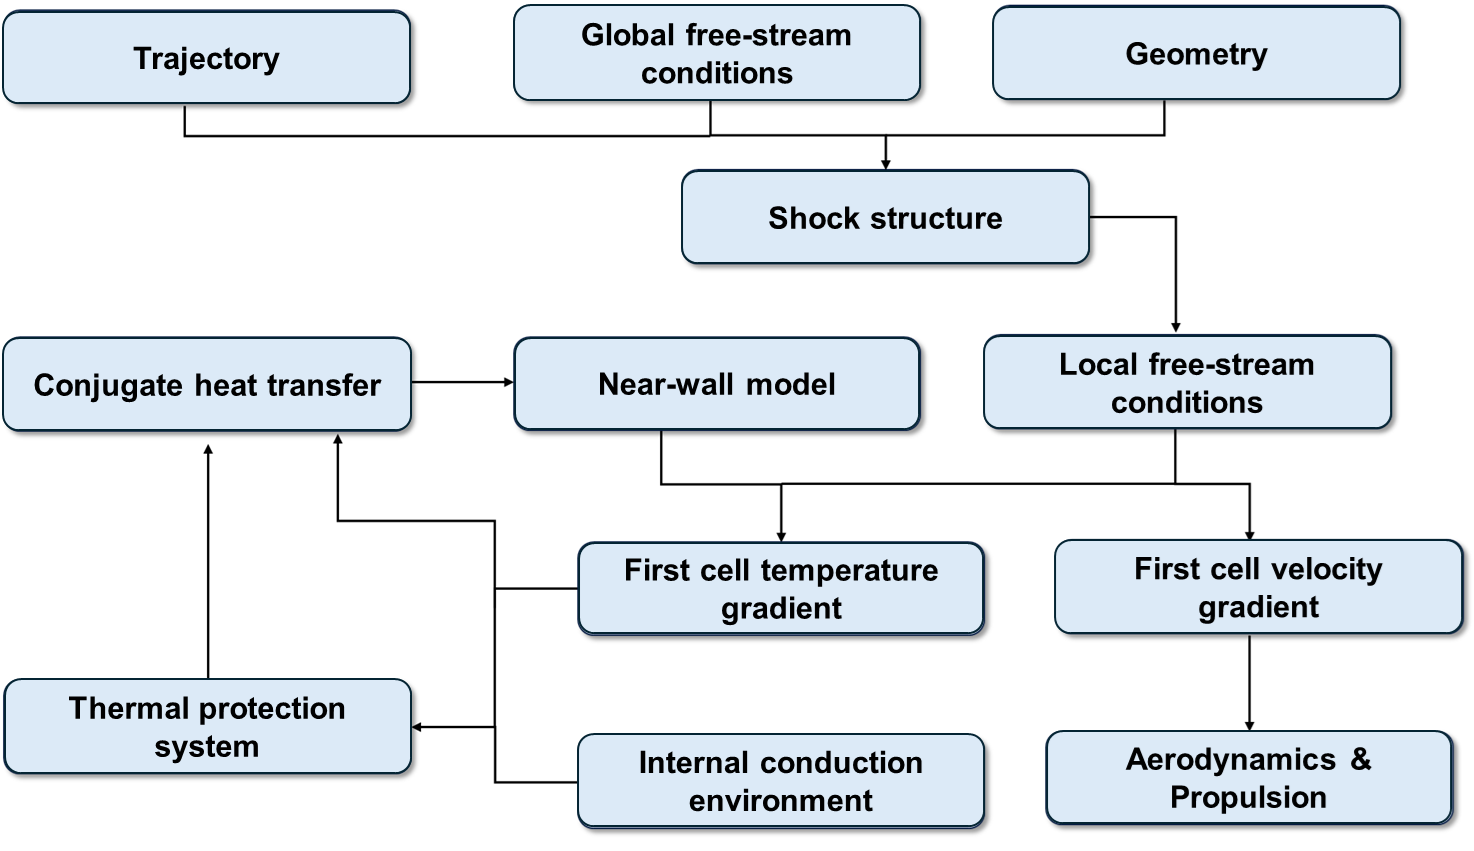
\includegraphics[width=1\linewidth]{flowchart.png}
\caption{Flowchart for low-order hypersonic aerothermal modeling}
\label{fig:1}
\end{figure}

For the direct calculation of aerothermal loading, there are three main user-defined inputs to the model, as shown in Figure~\ref{fig:1}: (1) trajectory (including initial conditions), (2) atmospheric conditions, and (3) vehicle geometry (including propulsion). In its current form, SUAVE utilizes these inputs to estimate the aerodynamic loads with the help of the vortex lattice method, along with propulsion parameters using one-dimensional formulations for propulsive subcomponents. The present work aims to extend the SUAVE framework to include an aerothermal module containing low-fidelity estimations of shock structure, surface heat flux, and temperature profiles. 
At each location along the trajectory, the shock structure on the vehicle can be computed and shock relations used to calculate the post-shock freestream conditions on the vehicle. With the appropriate wall modeling assumptions, along with a simplified assumption on the state of the boundary layer, near-wall thermal and kinematic states can be estimated. In conjunction with a conjugate heat transfer calculation, the gradient and heat flux on the vehicle can be estimated. These values can then be corrected by modeling the thermal protection efficacy. %Each of these submodels are discussed in the following subsection.

%\rw{quantify the uncertainty of the predictive modeling of aerothermal heating...}
%This paper will summarize the state-of-the-art in each subdiscipline and provide a roadmap for the development of a holistic predictive modeling framework with uncertainty quantification.

\subsection{Modeling of components}
To build modules to predict the aerothermal heating load, the following models are integrated into the SUAVE framework.

\subsubsection{Trajectory and atmospheric conditions}

Trajectory design is a key component in controlling the aerothermal heating of a hypersonic vehicle. For a reentry trajectory, entry point parameters such as coordinates, velocity, angle of attack, and inherent vehicle aerodynamics are critical in attaining the target flight profile. For a ground-based takeoff/landing mission, fuel margin, duration of hypersonic cruise, and vehicle aerodynamics are critical in reaching target range and altitude. In both cases, material constraints imposed by aerothermal heating is a limiting parameter. Considering the multi-parametric dependence of the target entity, an optimization framework is of high priority when designing hypersonic missions. %In this regard, the built-in multi-fidelity optimization feature in SUAVE, makes it an attractive tool for integrating and solving low-order models.
%developed by integrating an array of python optimization packages\citep{macdonald_suave_2017-1}

For the present work, a reentry trajectory module is added to the SUAVE framework, currently limited to an equilibrium glide trajectory, which assumes a very small descent angle. The velocity profile for an equilibrium gliding trajectory is estimated as:

\begin{equation}
    \frac{V}{V_e} = \left[1 + \frac{\rho R_0}{2\beta} \frac{L}{D} \right]^{-\frac{1}{2}}
    \label{equ_glide}
\end{equation}

where $R_0$ is the earth radius, $\rho$ is the free-stream density, $V_e$ is entry point vehicle velocity, $\beta$ is the ballistic coefficient of reentry and $L$/$D$ is the lift-to-drag ratio input to the model.

SUAVE estimates atmospheric conditions using a built-in atmospheric model up to 86~km, namely the 1976 US Standard Atmosphere \citep{united_states_committee_on_extension_to_the_standard_atmosphere_us_1976}. For the present work, two extensions to this model are implemented for altitudes up to 120~km: i) extending the 1976 US Standard Atmosphere; and ii) using the upper atmosphere data computed by \cite{schouler_ixv_2021}. By comparing results produced using these two models, the sensitivity of the SUAVE aerothermal models to the assumed upper atmosphere conditions can be gauged. For the data of Schouler et al. \cite{schouler_ixv_2021}, static pressure is calculated from temperature and density assuming an ideal gas.

%\rw{add in details about how we can use different models based on the flight regime at a specific point in the trajectory. E.g. reference Fig 11 from the Karl paper. Apply different models based on threshold criteria (e.g. Re, excitation and relaxation phenomena). Note that the implemented Sutton-Graves type model seems to assume convective heat transfer only, so peak shock layer temperatures must remain below some limit for this to be ok (10 000 K?)}

% See (https://encyclopedia.pub/entry/37190#:~:text=An%20approximate%20rule%2Dof%2Dthumb,layer%20temperature%20of%207800%20K.) that general rule of thumb is_shocklayer ~ U_entry (m/s).
%For example, Apollo reentry velocity ~ 11km/s and the post-shock temperature considering the real-gas effects was ~11000K
%For IXV, reentry velocity ~ 7500m/s hence the post shock temperature should be well below 10000K limit.

\subsubsection{Shock structure}
The most important characteristic for the estimation of the aerothermal heating is the identification of the shock structure in the vehicle. The true shock structure depends on flight characteristics (velocity, angle, Mach number), vehicle geometry, and atmospheric conditions. Although time-varying shock structures are critical, simplifications can be made for low-order calculations. 
It is evident from physics that the highest laminar heat flux over a vehicle during its hypersonic flight will be at the stagnation point. From a geometric perspective, the stagnation point is the farthest upstream point on the vehicle for a given angle of attack. Then, the shock structure around a vehicle geometry is determined from the three-dimensional hyperbolic shock structure formulations reported by Billig 1967. 
\begin{equation}
    (x-x_0) = R_{stag}~ + \Delta~ - R_c~\cot^{2}\theta~\left[\left(1+\frac{(z-z_{0})^{2}\tan^{2}\theta}{R_{c} ^{2}}\right)^{\frac{1}{2}} - 1\right]
    \label{shock_structure}
\end{equation}
Here, the stagnation radius, $ R_{stag}$ is estimated on the symmetric x-z plane of the vehicle using a circle formed from the stagnation point, and maximum and minimum vertical points, with its centre positioned at $(x_{0},z_{0})$. Note that the present model assumes zero or near-to-zero yaw angle, which is the case for most hypersonic trajectories. Approximating the vehicle to a spherical cone strucutre, the shock stand-off distance, $\Delta$, is then defined by the correlation,
\begin{equation}
    \Delta~ = 0.143~ R_{stag}~ exp\left(3.24/M^{2}\right)
\end{equation}
The hyperbolic radius of curvature, $R_{c}$ is given by the relation,
\begin{equation}
    R_{c} = 1.143~ R_{stag}~ exp\left[0.54/\left(M-1\right)^{1.2}\right]
\end{equation}
The shock angle, $\theta$, is defined by,
\begin{equation}
    \theta = \sin^{-1}\left(1/M\right)
\end{equation}
After estimation of $R_{stag}$ using Billig's shock structure formulation, the stagnation point aerothermal laminar heat flux for dissociated air is estimated based on the convective \citep{detra_generalized_1961, hirschel_thermal_2015}, radiative  \citep{hirschel_thermal_2015} and total stagnation heat flux (in $W/m^{2}$) correlation, given as:

\begin{equation}
    \dot{q}_{conv} = k_1 \left(\frac {\rho}{\rho_{SL}}\right)^{0.5} \left(\frac {V}{V_{co}}\right)^{3.15} \left(\frac {1}{R_{stag}}\right)^{0.5}
    \label{heat_flux_conv}
\end{equation}
\begin{equation}
    \dot{q}_{rad} = k_2 \left(\frac {\rho}{\rho_{SL}}\right)^{1.5} \left(\frac {V}{10^{4}}\right)^{12.5} R_{stag}
    \label{heat_flux_rad}
\end{equation}
\begin{equation}
    \dot{q}_{stag} = \dot{q}_{conv} + \dot{q}_{rad}
    \label{heat_flux}
\end{equation}

where $k_1 = 11.03\times 10^{7}$, $k_2 = 7.9\times 10^{11}$, $\rho_{SL} = 1.225$~kg/m$^{3}$, $V_{co} = 7950$ $m/s$, and $\rho$ and $V$ are the local freestream density and instantaneous vehicle velocity, respectively. The stagnation pressure is computed from the freestream normal shock relations. These conditions provide a basis for estimating the temporal and spatial heat flux profiles over a hypersonic reentry vehicle.

\subsubsection{Spatial heat flux distribution}
The stagnation point laminar heat flux can be extended spatially by approximating cosine law of local surface inclination angle (Lees 1956, Kemp 1959). The local inclination angle at each coordinate point on the vehicle is derived from the normal vector between the center of a sphere generated from four surrounding points around the coordinate point of interest. Following the cosine formulation used by Morgado et al, the spatial variation in laminar heat flux can be represented as a function of local surface inclination angle, $\phi$ by,
\begin{equation}
    \dot{q}_{lam} = \dot{q}_{stag}\left(0.1+0.9~\cos\phi\right)
    \label{cosine_law}
\end{equation}

Now, laminar to turbulence transition regimes are important in accurate estimation of heat flux over vehicle surface. Towards modelling these regimes, the present work refers to the trends of the laminar heat flux parameter on the fore-end surface of Orion test specimen subject to low enthalpy hypersonic flow \citep{hollis_aeroheating_2009}. The relationship between laminar to transitional and turbulent heat flux is extracted from the test results to arrive at the following conditional relation for spatial heat flux profile:

\begin{equation}
\dot{q} = 
\left\{
    \begin{array}{lr}
        \dot{q}_{lam}, & Re_\theta\ \leq 226\\
        \dot{q}_{lam}~[1 + \frac{2.5}{174}~(Re_\theta - 226)], & 226 < Re_\theta\ < 400 \\
        \dot{q}_{lam}~[3.5 + \frac{1.5}{400}~(Re_\theta - 400)], & Re_\theta\ \geq 400
    \end{array}
\right\}
\label{lam_turb_condition}
\end{equation}

where $Re_\theta$ is the Reynolds number based on momentum thickness. Momentum thickness is quantified based on Thwaites' method using potential-flow surface-velocity distribution over a sphere, \cite{White_fluids} %(Chapter~4): %eqn : 4-138 \& 4-193

\begin{equation}
    \begin{array}{lr}
        \theta = \frac{0.45\mu}{\rho U^{6}}\int_{0}^{\phi} U^{5}d\phi \\
        \\
        U = \frac{3}{2}~U_\infty~ \sin\phi\\
        \\
        Re_\theta = \frac{\rho U \theta}{\mu}
    \end{array}
\label{thwaites}
\end{equation}

The thermophysical properties of the fluid in Equation~\eqref{thwaites} are assumed to be temperature dependent. The shock layer temperature at stagnation point is considered in this regard, which is derived from normal shock relations. 
An empirical correction factor of 0.3 is applied to $Re_\theta$ which contributes to its validation with the test results as seen later %Figure~\ref{Re-28-hollis}. Since the product of velocity distribution and momentum thickness is a function of thermophysical properties (as seen in Equation~\eqref{thwaites}), this empirical correction factor can be associated with the thermophysical properties near the wall of the ambient fluid. The factor can be considered as a correction factor towards inaccuracies in near-wall dynamic viscosity, which increases strongly during hypersonic free-stream conditions.

Finally, it must be noted that the surface heat flux formulations in Equation \eqref{lam_turb_condition} is derived from low enthalpy hypersonic test conditions, however, the laminar spatial heat flux distribution is based on cosine law applicable to high enthalpy conditions (Lees 1956, Kemp 1959). Regardless, a non-dimensional parameter, $Re_{\theta}$, is used to define the conditional transition to turbulence over the vehicle surface and hence the low-fidelity formulation is applicable to high enthalpy reentry conditions.

%\subsubsection{Near-wall modeling}
%The computation of the post-shock state over the vehicle provides the relevant conditions encountered by the vehicle. Predictive modeling of wall-bounded flows is based on the accurate computation of local velocity and temperature gradients at the wall. Although many correlations may provide wall temperature estimates based on the freestream (post-shock) state, many of these estimates break down under non-adiabatic wall conditions \citep{griffin_velocity_2021}. Many recent works have advanced the state-of-the-art in non-adiabatic high-speed wall modeling \citep{griffin_velocity_2021,younes_mean_2023,younes_velocity_2021}. These wall models can be integrated into the low-order modeling in order to improve the prediction for complex aerothermal heating conditions.


\subsubsection{Surface temperature solution}
Heat transfer characteristics in aerothermal heating are critical to the development of thermal management systems. In addition to the external aerothermal loads, hypersonic systems generate a significant amount of heat through tightly integrated propulsion systems and will likely carry internal heat-generating electronic components. Managing combined vehicle heat loads is critical to maintaining vehicle integrity and protecting thermosensitive equipment. A recent review of numerical modeling of aerothermal heating \citep{lewis_conjugate_2023} highlights the complexity of accurate predictions due to the strong coupling between phases, further strengthening the need for accurate wall models.   In the present work, heat transfer to the vehicle is modeled as a one-dimensional, one-way coupled, analytical system. This simplification abstracts from the geometrical complexity and conjugate heat coupling, but enables a nimble heat flow prediction. The analytical solutions for unsteady boundary conditions are estimated using Duhamel's method (Groulx 2009). \\
Consider a one-dimensional transient temperature profile, $T(x,t)$ within a material with length, $L$, thermal diffusivity, $\alpha$ and thermal conductivity, $k$. Then, the one-dimensional transient heat conduction through the material, subject to time varying heat flux, $\dot{Q}(t)$, can be mathematically written in non-dimensional form as,
\begin{equation}
    \begin{array}{lr}
        \dfrac {\partial \overline{T}}{\partial \overline{t}} = \dfrac {\partial^{2} \overline{T}}{\partial \overline{x}^{2}} \\
        \\
        \overline{T}(0,\overline{t}) = 0; ~ \dfrac {\partial \overline{T}}{\partial \overline{x}}(1,\overline{t}) = \overline{\dot{Q}}(t); ~ \overline{T}(x,0) = 0  \\ 
        \\
        \overline{T} = \dfrac {(T-T_0)~k}{\dot{Q}(0)~L}; ~ \overline{x} = \dfrac {x}{L}; ~\overline{t} = \dfrac {\alpha~t}{L^{2}}; ~  \overline{\dot{Q}}(t) = \dfrac{\dot{Q}(t)}{\dot{Q}(0)} = 1 + \dfrac{S(t)~\delta t}{\dot{Q}(0)}
    \end{array}
    \label{duhamel}
\end{equation}
where $S(t)$ is the instantaneous slope of input heat flux profile in a time interval $\delta t$. According to Duhamel's theorem, the solution to this problem, that is the temperature at any point in the material, can be found using superposition of solutions to a similar problem with piecewise-linear variation in heat flux. Then, the solution to the Equation \eqref{duhamel} at time $t$, having $M$ piecewise-linear segments in input heat flux profile, using Duhamel's theorem will lead to a temperature distribution inside the material expressed as;
\begin{equation}
    \begin{array}{lr}
        T(x,t) = \left[\sum\limits_{i=1}^{M} \left(\Delta T_a~ + ~\Delta T_b\right)~\right] + T_0\\
        \\
        \Delta T_a~ = 
        \left\{
            \begin{array}{lr}
                \dfrac{\left(\dot{Q}_{i-1}~ - ~\dot{Q}_{i-2}\right)~k}{k}~\left[\dfrac{x}{L}+\sum\limits_{n=1}^{\infty} A_n~\Phi_n(x)~exp\left[-\lambda_{n}^{2}~(Fo(t) - Fo(t_{i-1}))\right]\right], & i > 1  \\
                \\
                \dfrac{\dot{Q}_{0}~k}{k}~\left[\dfrac{x}{L}+\sum\limits_{n=1}^{\infty} A_n~\Phi_n(x)~exp\left[-\lambda_{n}^{2}~Fo(t)\right]\right], & i = 1
            \end{array}
        \right\}\\
        \\
        \Delta T_b~ = \dfrac{\left(\dot{Q}_{i}~ - ~\dot{Q}_{i-1}\right)~L}{Fo(t_i)~k}~\left[Fo(t_i)+\sum\limits_{n=1}^{\infty} \dfrac{A_n}{\lambda_{n}^{2}}~\Phi_n(x)~exp\left[-\lambda_{n}^{2}~Fo(t_i)\right]~\left\{1-exp\left[-\lambda_{n}^{2}~Fo(t_i)\right]\right\}\right]\\
        \\
        A_n = \dfrac{2(-1)^{n}}{\lambda_n};~ \Phi_n(x) = \sin\left(\lambda_n~\dfrac{x}{L}\right);~ Fo(t) = \dfrac {\alpha~t}{L^{2}};~ \lambda_n = \dfrac{(2n-1)}{2}~n\pi
    \end{array}
    \label{surface_temperature}
\end{equation}
Finally, the temperature at each surface point over the vehicle, at which the transient aerothermal heat load exists, can be computed by substituting $x=L$ in Equation \eqref{surface_temperature}. This temperature profile at each time instance is checked iteratively for heat balance between aerothermal heating, $\dot{q}$, surface radiative cooling, $\dot{q}_{r}$ and material conduction $\dot{Q}$, through all points on vehicle surface:
\begin{equation}
    \begin{array}{lr}
        \dot{Q} = \dot{q} - \dot{q}_{r}\\
        \dot{q}_{r} = 5.67\times 10^{-8}~\times T^4(L,t)
    \end{array}
    \label{heat_balance}
\end{equation}

Key limitations to the current surface temperature estimation methodology include one-dimensionality, restriction of using temperature-independent properties, and lack of boundary layer feedback or conjugate heat transfer.



\section{Validation Cases}

To validate the low-order near-wall model for hypersonic aerothermodynamics, simple geometries are chosen, for which experimental results and analytical solutions of well-characterized bow shocks are readily available in the open literature. %Two cases are being considered for this work, each of which are based on results from experimental wind tunnel tests. 

\subsection{Orion experiments}

For this work, the results of the experimental investigation of the Orion crew exploration vehicle (CEV) by \cite{hollis_aeroheating_2009} are used to validate the spatial variation in the predicted aerothermal heat loads using the present SUAVE model. Experiments were conducted using gaseous nitrogen as the test gas on a scaled down test specimen of Orion CEV. Tests carried out for Mach numbers at 7.5 and 10, over angles of attack of 24$\degree$, 28$\degree$ and 32$\degree$ are considered as validation cases. As the results show good agreement on the general trends between the three angles of attack, the analysis focuses on the 28$\degree$ cases; the other cases are presented in the appendix. The test conditions at 28$\degree$ are summarized in Table~\ref{hollis_test_inputs}. 

\begin{table}[hbt]
\caption{Test conditions for 28$\degree$ angle of attack from \cite{hollis_aeroheating_2009}}
\label{hollis_test_inputs}
\begin{center}
\begin{tabular}{c c c c c c c}
 \textbf{$V_\infty(\frac{m}{s})$} & \textbf{$\rho_\infty (\frac{kg}{m^{3}})$} & \textbf{$P_\infty (Pa)$} & \textbf{$M_\infty$} & \textbf{$T_{wall} (K)$} & \textbf{$H_0 - H_{300K} (\frac{J}{kg})$} & \textbf{$Re_\infty (\frac{1}{m})$}\\ 
\hline\\
1300 & 0.105 & 2280 & 7.45  & 320  & 6.10e5 & 2.7e7 \\
 1410 & 0.225 & 5570 & 7.57 & 386  & 7.69e5  & 5.5e7 \\
 1367 & 0.378 & 8290 & 7.80 & 382  & 6.99e5  & 10e7 \\
 1473 & 0.110 & 1610 & 10.3 & 325  & 8.69e5  & 4.8e7 \\
 1478 & 0.148 & 2120 & 10.4 & 336  & 8.31e5  & 6.5e7 \\
% \hline
\end{tabular}
\end{center}
\end{table}

\subsubsection{Shock structure}
Given that the capsule is at an angle of attack, it is assumed that the stagnation point is the farthest upstream point on the vehicle under the corresponding flight condition. The stagnation radius is estimated on the symmetry plane using a circle formed from the stagnation point, and maximum and minimum vertical points on the plane. The three-dimensional shock structure is estimated using Equation \eqref{shock_structure} and is shown in Figures~\ref{shock2d} and \ref{shock3d}.

\begin{figure}[h!]
\centering
\begin{subfigure}[b]{0.49\textwidth}
\centering
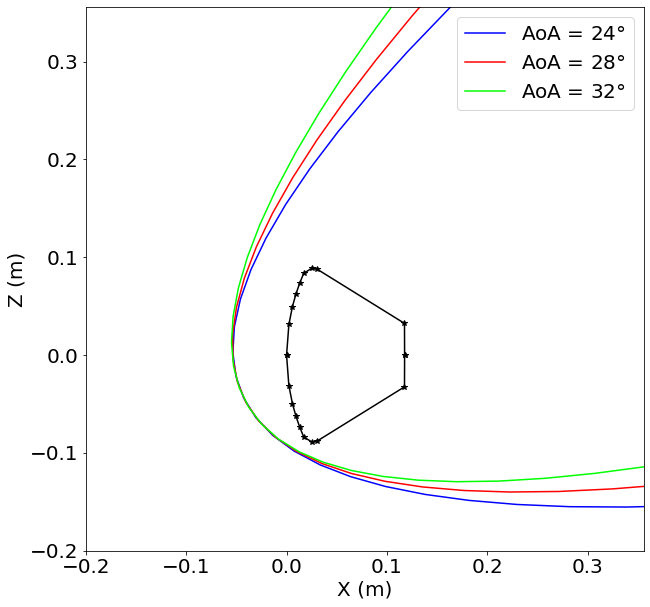
\includegraphics[width=\textwidth]{shock2D.png}
\caption{2D shock structure}
\label{shock2d}
\end{subfigure}
~
\begin{subfigure}[b]{0.49\textwidth}
\centering
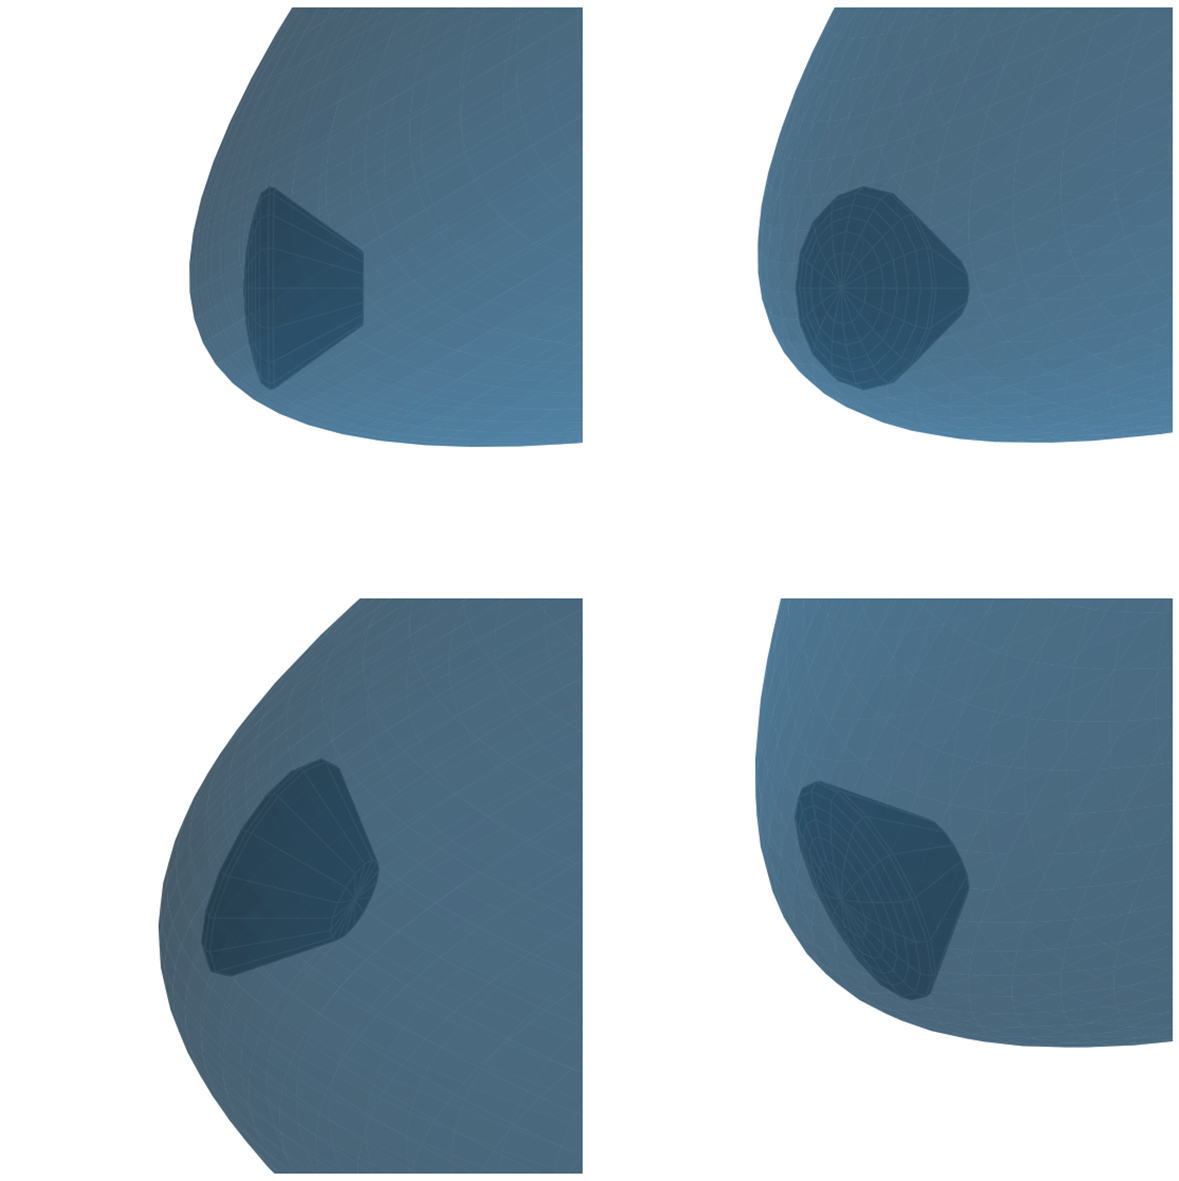
\includegraphics[width=\textwidth]{shock3D.png}
\caption{3D shock structure isometric views at 28$\degree$ angle of attack}
\label{shock3d}
\end{subfigure}
\caption{Multi-dimensional depiction of shock structure around Orion test specimen}
\end{figure}

It can be seen in Figure~\ref{shock2d} that the shock stand-off distance near the stagnation point is very small. %Note that at very high Mach numbers, shock formation close to the vehicle surface can lead to intense shock radiation, resulting in an amplified surface heat flux. 
It is noted here that the estimation of shock stand-off distance is critical in establishing radiation from the shock structure, which is accountd for in form of Equation \eqref{heat_flux_rad}.

\subsubsection{Spatial heat flux distribution}
The surface heat flux model is based on the stagnation point laminar heat flux extended over the surface using cosine function which conditionally transitions into turbulent heat flux levels as per Equations \eqref{cosine_law}-\eqref{thwaites}. Sutherland's law is used to estimate the temperature-dependent viscosity and thermal conductivity of the working fluid, nitrogen in this experimental case \citep{White_fluids}, and its specific heat is estimated from the temperature-dependent correlation of \cite{Chase_NIST}. Figure~\ref{Re-28-hollis} shows the comparison of $Re_{\theta}$ profile over the mid plane fore-end surface of Orion test specimen. 

\begin{figure}[h!]
\centering
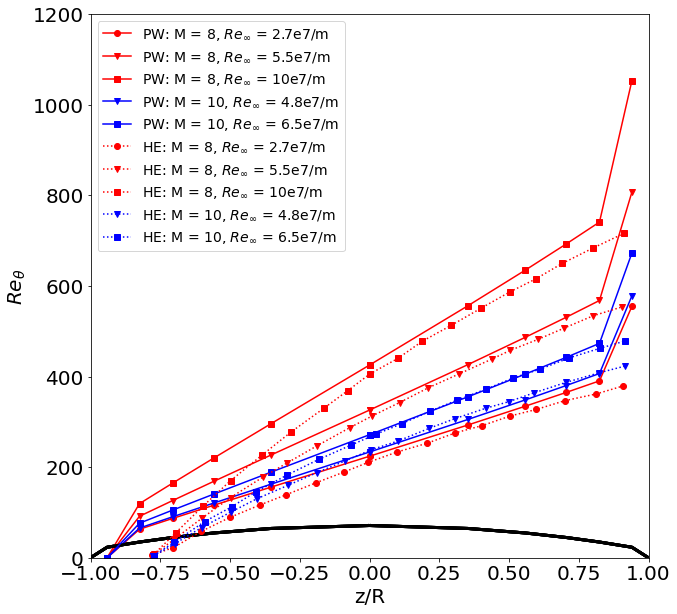
\includegraphics[width=0.7\linewidth]{Re-28-hollis.png}
\caption{$Re_\theta$ vs normalized capsule height at 28$\degree$ angle of attack. HE: Hollis et al Experiment, PW: Present Work}
\label{Re-28-hollis}
\end{figure}

It can be seen in Figure~\ref{Re-28-hollis} that the $Re_\theta$ predicted by the model follows well with that reported in \cite{hollis_aeroheating_2009}. The predicted stagnation point is observed to be further away from the capsule centerline in comparison with the reported value. This is also observed for the 24$\degree$ cases, shown in the appendix. Due to this shift, there exists a mismatch in $Re_\theta$ close to the stagnation point. However, this will have minimal impact on surface heat flux predictions, as the laminar value (independent of $Re_\theta$) is applied close to the stagnation point and very good agreement is generally observed away from this region for $Re_\theta > 300$. 
%Note: since the crew module fore-end sphere half angle is 23 deg, it is logical any angle of attack above 23 deg should be in the corner of the fore-end (refer Morgado paper figure 4). Model captures this, but test results shows otherwise.

With the validation of Reynolds-based momentum thickness distribution, the surface heat flux along the symmetry plane of the Orion CEV test specimen is estimated based on Equation \eqref{lam_turb_condition}. This is presented and compared with test results in Figure~\ref{St-28-hollis} based on a corrected Stanton number, which accounts for variations of the Reynolds number and the effects of different enthalpy levels in various experimental facilities \citep{hollis_aeroheating_2009}:

\begin{equation}
    St\cdot Re_{\infty,D}^{1/2} = \frac{\dot{q}} {\rho_\infty V_\infty \left[\sqrt{Pr}~ H_0 - H_{wall}\right] } \left(\frac{\rho_\infty V_\infty D}{\mu_\infty}\right)^{\frac{1}{2}}
    \label{lam_param}
\end{equation}

%would deem the surface heat flux to be independent of the transience in surface temperature profile. 
%Further, the paper concludes that at the start of the turbulent regime, the laminar correlation parameter is augmented by 3.5 times over the fore-end side of crew module and further increases linearly as a function of Reynolds number based on momentum thickness ($Re_\theta$).  %is  a turbulent heat transfer augmentation of up to 5.5 times, compared to laminar values, for the laminar correlation parameter of $St\cdot Re_{\infty,D}^{1/2}$, which accounts for variability during experiments.

%Surface heat flux over the mid-plane of Orion crew module is predicted using the model developed in SUAVE and compared with laminar correlation parameter for surface heat flux as shown in Figure \ref{St-28-hollis}. Data from the 24$\degree$ and 32$\degree$ cases are presented in the appendix.

\begin{figure}[h!]
\centering
\begin{subfigure}[b]{0.49\textwidth}
\centering
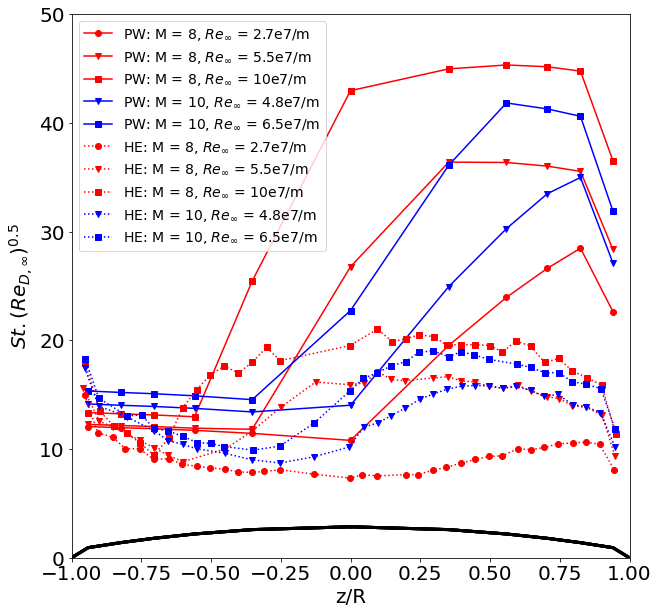
\includegraphics[width=\textwidth]{St-28-hollis.png}
\caption{Original correlation of \cite{hollis_aeroheating_2009}}
\label{St-28-hollis}
\end{subfigure}
~
\begin{subfigure}[b]{0.49\textwidth}
\centering
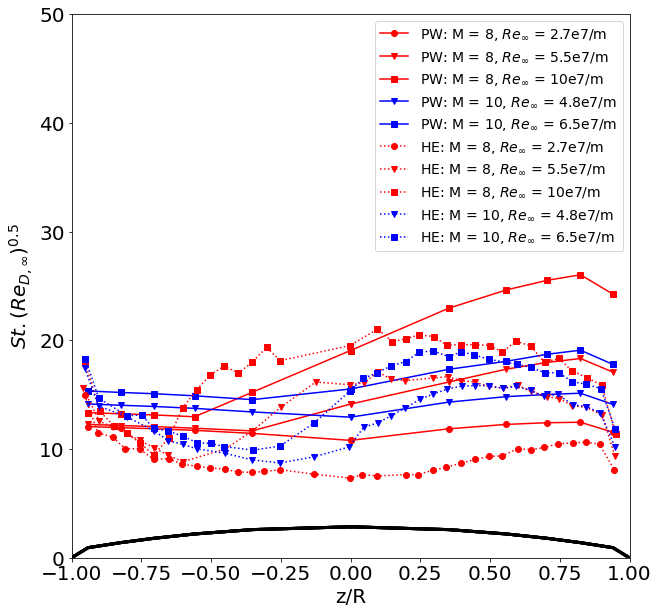
\includegraphics[width=\textwidth]{St-28-hollis-new.png}
\caption{Modified correlation}
\label{St-28-hollis-new}
\end{subfigure}
\caption{Normalized heat flux vs normalized test specimen height at 28$\degree$ angle of attack. HE: Hollis et al Experiment, PW: Present Work}
\end{figure}

It can be seen in Figure~\ref{St-28-hollis} that, even though the onset of the transition is captured fairly well by the model, the transition and turbulent heat flux parameters are clearly too high in each case. The figure also shows that the laminar heat flux parameter drops gradually compared to the sudden dip in the measured parameter close to the stagnation point. Both of these observations can be attributed to the cosine law formulation of the surface heat flux profile. The fraction of stagnation heat flux near $z/R = 1$ is calculated to be approximately 0.7 using the cosine law, while the reported fraction is only 0.4. This difference in the stagnation heat flux fraction results in amplified surface heat flux predictions in the turbulent regime. In addition, the cosine gradient around the zero inclination angle is nearly zero, resulting in the overprediction of surface heat flux near the stagnation point. Now, it has already been mentioned that cosine law is specific to high enthalpy hypersonic flows, hence the inaccuracies in results while comparing cosine law with low enthalpy hypersonic test conditions are expected. 

In order to obtain better predictions for transition and turbuelnt regimes, Equation~\eqref{lam_turb_condition_new} is modified in the present work as follows:

\begin{equation}
\dot{q} = 
\left\{
    \begin{array}{lr}
        \dot{q}_{lam}, & Re_\theta\ \leq 226\\
        \dot{q}_{lam}[1 + \frac{0.5}{174}(Re_\theta - 226)], & 226 < Re_\theta\ < 400 \\
        \dot{q}_{lam}[1.5 + \frac{1.5}{400}(Re_\theta - 400)], & Re_\theta\ \geq 400
    \end{array}
\right\}
\label{lam_turb_condition_new}
\end{equation}

Applying Equation~\eqref{lam_turb_condition_new}, the surface heat flux along the capsule symmetry plane is recalculated and compared to the experimental values in Figure~\ref{St-28-hollis-new}.

With the updated correlation in the transitional and turbulent regimes, the surface heat flux profile over the symmetry plane forebody region of the Orion CEV test specimen is fairly well represented. The onset of transition remains intact from the original correlation, whereas the transition and turbulent heat flux parameters are predicted within the error bounds of cosine law formulation, as seen in Figure~\ref{St-28-hollis-new}. It is noted here that the turbulent heat flux prediction error is minimal for $Re_\infty \thicksim 5e7/m$ and the error increases on either side of this $Re_\infty$. This is because the local heat flux and its enhancement in transition regime is not accurately captured by the cosine law, leading to a shift in the skewness of errors as $Re_\infty$ increases. Even though errors persist in the cosine law model, it provides a good estimation of the order of magnitude of surface heat flux under high-speed flow conditions. Hence, the surface heat flux estimation methodology with updated conditions is used in further predictions using the model.
%The first bow shock validation case is the work of \cite{menezes_experimental_2003}, who experimentally investigated the Stanton number distribution over the front end of a 120$\degree$ blunt cone, having a 25~mm nose radius and 100~mm total span. Testing was conducted using air as the test gas at a nominal freestream condition of Mach 5.75 and static temperature of 140~K. The model was tested at 0$\degree$, 7$\degree$  and 12$\degree$  angle of attack. 

%The first case is the investigation of the Orion crew exploration vehicle aerothermal heat loads by \cite{hollis_aeroheating_2009}. Tests were conducted for Mach numbers from 7.5--10.5 over a range of angles of attack and static temperatures around 60~K. The authors demonstrated a turbulent heat transfer augmentation of up to 5.5 times, compared to laminar values, for the laminar correlation parameter of $St\cdot Re_{\infty,D}^{1/2}$, which accounts for variability during experiments. 

%The laminar heat transfer profile across the blunt nose section was represented by the correlation $St\cdot Re^{1/2}$ and turbulent heat transfer profile by $St\cdot Re^{1/5}$. The ratio of these correlations, called turbulent augmentation factor, shows that turbulent heat transfer rates at aft end of the vehcile is amplified by 5.5 times compared to laminar heat transfer rates. 
%they normalized the data in this way to account for fluctuations in freestream conditions (5%) and model surface temperature increasing 150 K over an experiment - let's wait and see if we need to make use of this. 

%The final test case is that of \cite{liu_experimental_2013}, who investigated the surface heat flux over a Mach 10 blunt-nosed waverider configuration, with a nose radius of 30~mm, and total body length and height of 352~mm and 129~mm, respectively. A key result for comparison is an 80\% reduction in surface heat flux from peak values at distances over 10\% of the total vehicle length for -3$\degree$ to 6$\degree$ angles of attack. 

%\subsection{Shock-shock interaction}
%Estimation of the shock structure over the vehicle during its hypersonic trajectory is key in understanding the localized surface heat fluxes. While simpler geometries exhibit simple bow shocks under hypersonic compression, full scale hypersonic vehicles with complex geometries and appendages would exhibit shock-shock interactions and shock-wall interactions. As the vehicle maneuvers, such interactions would cause transience in local boundary layer profile and surface heat flux profile. Thus, validation of shock structure model and resulting effects on surface heat flux is necessary. 
%Shock-shock interaction can take several structures as mentioned in the literature work by \citep{edney_anomalous_1968}. Type III (a supersonic jet and a shear layer) and type IV (two supersonic jet) interactions were tested by \citep{wieting_multiple_1992}, by impinging oblique shock interference from double wedge onto 76mm diameter cylinder. For a free-stream air temperature of 125~K and Mach 8, the resulting surface heat flux was found to be upto 38 times the undisturbed-flow stagnation-point heat flux. Additionally, several validation cases can be extracted from the review work by \citep{holden_review_1997} in which the surface heat flux profiles due to shock-shock interactions over simple geometries for Mach 6 to 18 in rarefied to fully continuum turbulent flow regimes are extensively reviewed. 

%\subsection{Apollo reentry mission}

%However, experimental studies on hypersonic conjugate heat transfer are limited \citep{lewis_conjugate_2023}.
%Instead, a generic reentry mission of Apollo crew capsule is used as validation point here. 
%\textit{ FORMER CONTENT: As experimental studies on hypersonic conjugate heat transfer are very limited \citep{lewis_conjugate_2023}, an analytical reference work is to be used for validation. \cite{ko_reentry_2007} investigated a generic reentry mission of the Apollo crew capsule, using a ballistic reentry trajectory and presenting the stagnation point heat-flux profile along with thermophysical material properties. 
%Comparison will be limited in the present work to the non-ablative thermal analysis, for which the thermal protection system strucutre consists of a passive thermal protection pad and inner sandwiched composite honeycomb.
%The maximum surface temperature of the thermal protection pad is reported to be 1965~K, while the temperature at the sandwich panel away from the pad maintained a temperature of 294~K throughout the mission. Considering the post-shock temperature of 11,000~K, radiation from the bow shock becomes significant, enabling analysis of the effects of the radiation model in Equation~\eqref{heat_flux_rad} of the results.}

 %Using the aerothermal module mentioned in the previous section, the spatial heat flux distribution over the forebody of the hypersonic vehicle can be estimated. In this section, the spatial heat flux distribution is used to estimate the spatial temperature distribution using analytical solutions for one-dimensional transient conduction through the vehicle thickness in Cartesian coordinates. 
 
%In this regard, the Apollo 9 crew exploration mission is used as a test case. The trajectory and material properties (Apollo TPS material of thickness 7.1cm and thermophysical properties evaluated at 1177K) of the crew exploration vehicle (CEV) are taken from \cite{ko_reentry_2007}. The analytical solution is derived using Duhamel's theorem, which approaches the solution to the spatial temperature profile due to a time-dependent boundary condition through superposition of a time series of solutions to the problem with piecewise time-independent boundary conditions~\cite{groulx2010analytical}. 

%In the present case, the time-varying heat flux represents the boundary condition at the fore-end of the CEV and an isothermal boundary condition (300 K) is assumed at its inner wall. The surface is allowed to cool radiatively to arrive at a heat balance at each temporal point. Based on the heat flux prediction for the Apollo CEV, the temporal variation in stagnation point temperature is shown in Figure~\ref{Apollo_stagnation}. The spatial variation in temperature over the symmetry plane of the Apollo CEV forebody is shown in Figure~\ref{Apollo_surface}.
%\begin{figure}[h!]
%\centering
%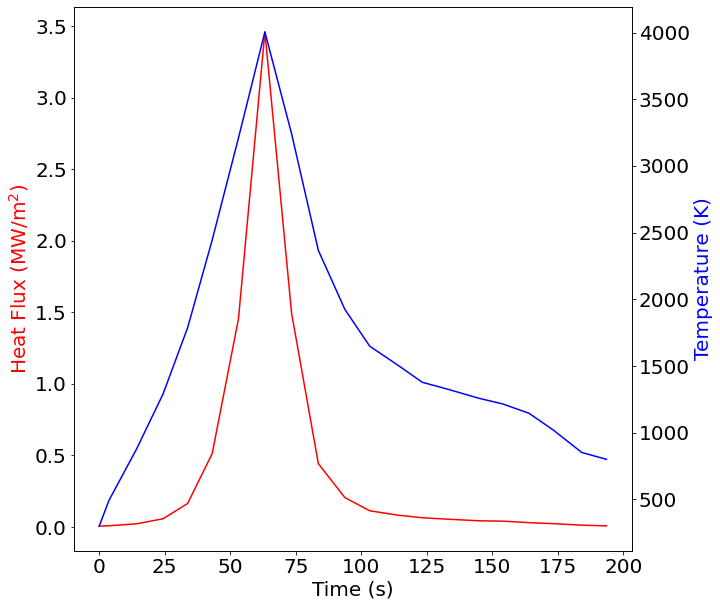
\includegraphics[width=0.7\linewidth]{Apollo_stag_point.png}
%\caption{Stagnation point heat flux and temperature history predictions for Apollo 9 CEV}
%\label{Apollo_stagnation}
%\end{figure}
%\begin{figure}[h!]
%\centering
%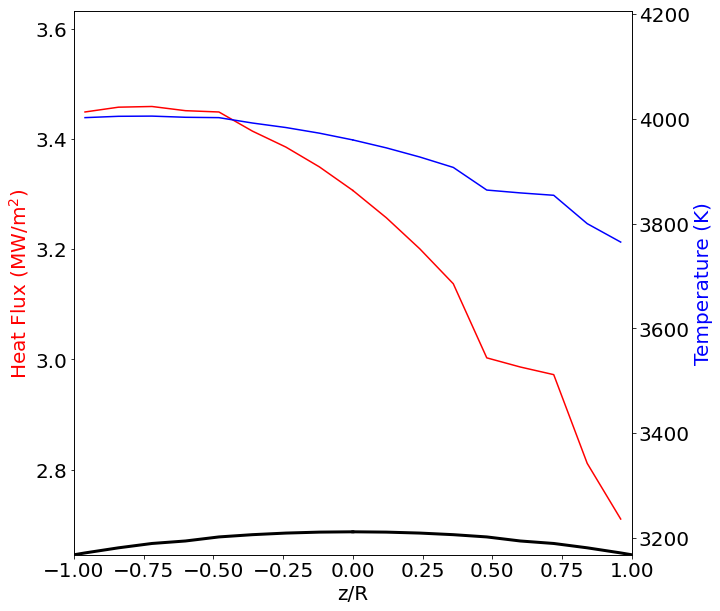
\includegraphics[width=0.7\linewidth]{Apollo_surface_thermal.png}
%\caption{Fore-end surface heat flux and temperature profile predictions for Apollo 9 CEV at 63s from the start of reentry}
%\label{Apollo_surface}
%\end{figure}

%From Figure~\ref{Apollo_stagnation}, the peak heat flux value is predicted to be $3.45MW/m^{2}$ occurring at 63s from start of atmospheric reentry, against the reported values of $1.86MW/m^{2}$ and 66s \cite{lee1972apollo}. Eventhough the timing of peak heat flux occurrence is matched well with value reported in literature, the overprediction of heat flux can be attributed to the absence of elaborate formulations for multi-physics involved with high-speed reentry scenario such as high enthalpy effects and entropy variation effects due to blunt body. It is also noted that the peak stagnation point temperature is predicted to be 4000 K against a measured value of 2200 K, even after considering radiative cooling for the surface. The overprediction of the stagnation point temperature can be attributed to several physical aspects, not modeled here, that can occur at very high temperatures such as surface ablation and ionization effects. These aspects are endothermic processes and hence can significantly lower the surface temperatures from the values predicted using the model.

%From Figure~\ref{Apollo_surface}, the drop in heat flux across the fore-end surface from stagnation point is predicted by the model, keeping in mind the limitations of the spatial heat flux formulations mentioned in the previous section. 
%It should also be noted here that the increase in aerothermal heat flux as a result of the variation in surface temperature is not currently formulated. This conjugate heat transfer (CHT) effect is essential to improve the accuracy of overall aerothermal predictions. The CHT can be achieved in the present model by replacing the empirical formulations for aerothermal heating with near-wall boundary layer models. Furthermore, the assumption of one-dimensional heat conduction within the vehicle is considered reasonable given the significant temperature difference between its outer and inner surfaces; however, improved accuracy is expected by considering spatial heat conduction solutions. 

\subsection{IXV reentry mission}
The Intermediate eXperimental Vehicle (IXV) was developed by the European Space Agency and successfully tested controlled reentry from Low Earth Orbit in February 2015 \citep{haya-ramos_design_2016}. Critical aerothermal parameters, including stagnation point heat flux and pressure profiles, were recorded throughout the trajectory, from reentry at 120~km altitude until parachute deployment at 25~km. 

The IXV reentry flight was simulated within the current low-order model framework, and the results were validated against the measured mission profile, deceleration profile, and aerothermal heating. A simplified geometry of the IXV, shown in Figure~\ref{model}, was developed for use in SUAVE using fuselage coordinate points derived from the IXV reference geometry mentioned by \cite{haya-ramos_design_2016}.

\begin{figure}[ht]
\centering
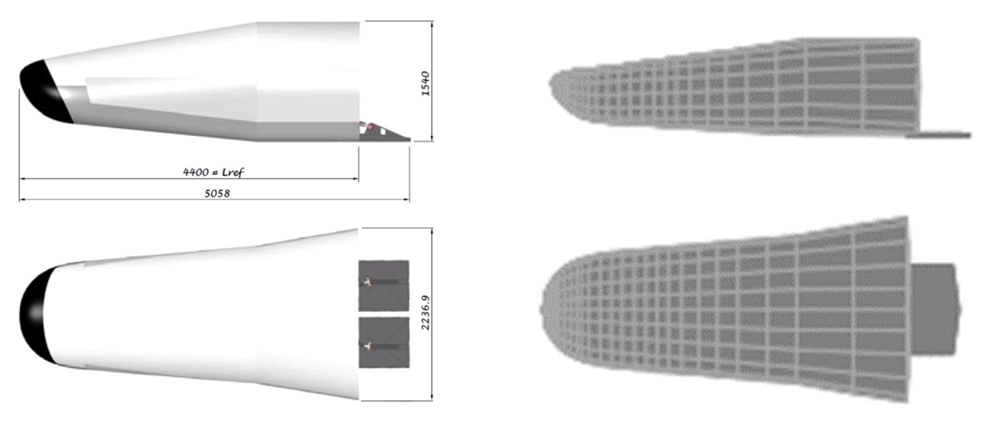
\includegraphics[width=1\linewidth]{IXV_model.png}
\caption{IXV reference geometry \citep{haya-ramos_design_2016} vs SUAVE rendered geometry}
\label{model}
\end{figure}

The input of the model to predict the IXV mission is shown in Table~\ref{IXV_inputs}. In actual flight, the angle of attack was maintained at 45$\degree$, however, the descent angle for IXV \citep{blau_ixv_2018} varied between 1.2$\degree$ and zero during the initial 1000s of reentry, followed by a sharp increase of up to 6$\degree$ until the deployment of the parachute at 1250s. Note that a descent angle of 1.2$\degree$ is small enough to assume a gliding trajectory. In addition, integrating Equations~\eqref{equ_glide}, \eqref{heat_flux}, predictive surface heat flux and temperature formulations, as well as built-in aerodynamic modules, SUAVE predictions are made for the IXV reentry flight. 

%However, since this affects the stagnation point nose radius from equation~\ref{heat_flux}, a the nose radius shown in Table~\ref{IXV_inputs} are digitially found from IXV geometry at its mid point (angle of attack = 45$\degree$). }

\begin{table}[ht]
\caption{Parameters for developing SUAVE model of IXV, taken from \cite{pezzella_aerodynamic_2014,goncalves_hypersonic_2020}}
\label{IXV_inputs}
\begin{center}
\begin{tabular}{l c}
\textbf{Parameter} & \hspace{2em} \textbf{Value} \hspace{2em} \\ 
\hline \\
\textbf{Vehicle:} &  \\
\cline{1-1}
Length [m] & 4.4 \\
Maximum height [m] & 1.5 \\
Width [m] & 2.2 \\
Flap length [m] & 0.66  \\
Nose radius [m] & 0.834  \\ \\
\textbf{Mission:} &  \\
\cline{1-1}
Entry velocity [m/s] & 7450 \\
Entry altitude [km] & 120 \\
Ballistic coefficient [kg/m$^{2}$]  &  690.71  \\
${L}$/${D}$ ratio & 0.7 \\
Angle of attack [$\degree$] & 45 \\
Final altitude [km] & 25 \\
% \hline
\end{tabular}
\end{center}
\end{table}

\subsubsection{Aerodynamic results}
The mission profiles of two simulation cases using (A) \cite{schouler_ixv_2021} and (B) US Standard Amospheric data extended to 120 km altitude \citep{united_states_committee_on_extension_to_the_standard_atmosphere_us_1976}, are shown in Figures~\ref{valid1}. The cases are executed considering an average descent angle of 1.2$\degree$.

\begin{figure}[h!]
\centering
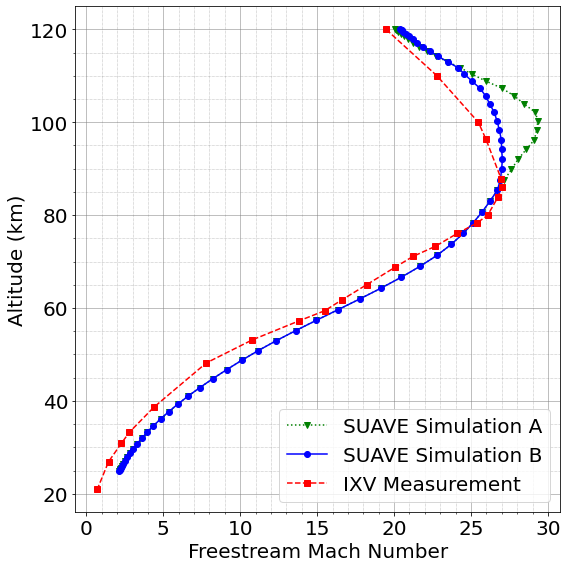
\includegraphics[width=0.5\linewidth]{IXV_mission_profile_1976.png}
\caption{Comparison of measured vs SUAVE simulated IXV mission profile}
\label{valid1}
\end{figure}

It is clear from Figure~\ref{valid1} that the Mach number profile during the upper atmosphere phase of reentry is highly dependent on the assumed atmospheric model, specifically the temperature data. It is also evident from Figure~\ref{valid1} that the freestream density plays a key role in upper atmosphere heat flux predictions, as per Equation~\eqref{heat_flux}.

As seen in Figure~\ref{valid1}, at the point of parachute deployment, the IXV had a final Mach number of 1.5, while the SUAVE model predicted a value of Mach 2.2. The trajectory simulated by SUAVE has a duration of 22 minutes from reentry to the parachute deployment point, compared to the actual mission duration of 21 minutes (not shown). Overall, the predicted mission profile matches well with flight data, but the Mach number is generally overpredicted, particularly above 90~km. This trend is observed to vary as the input descent angle is varied, as seen in Figure~\ref{valid2_1}, generated using extended 1976 US Standard Atmospheric data.
\begin{figure}[ht]
\centering
\begin{subfigure}[b]{0.49\textwidth}
\centering
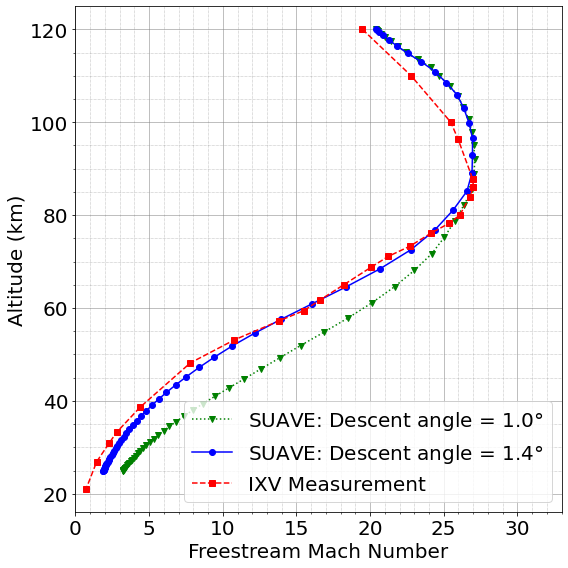
\includegraphics[width=\textwidth]{IXV_mission_profile_1976_1.png}
\caption{Mission profile}
\label{valid2_1}
\end{subfigure}
~
\begin{subfigure}[b]{0.49\textwidth}
\centering
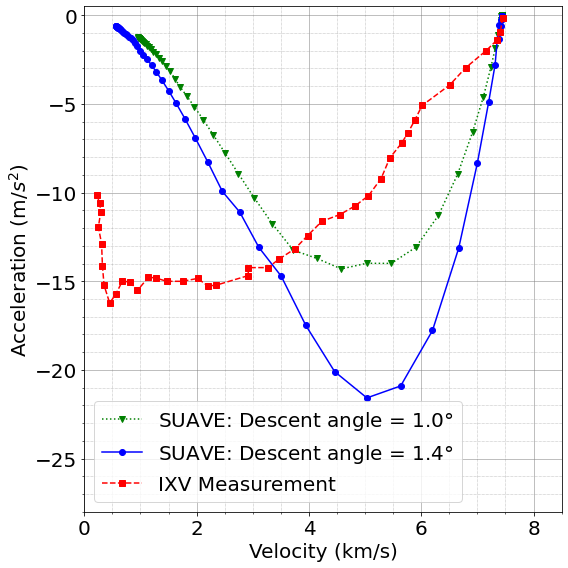
\includegraphics[width=\textwidth]{IXV_deceleration_1976.png}
\caption{Acceleration profile}
\label{valid2_2}
\end{subfigure}
\caption{Comparison SUAVE simulated IXV parameters at different descent angles vs IXV measurement}
\label{valid2}
\end{figure}

As expected, the peak initial velocity from Figure~\ref{valid2_1} matches well, but the SUAVE results show an earlier peak deceleration, as seen in Figure~\ref{valid2_2}, while the vehicle still has a velocity of around 5~km/s. The magnitude of the deceleration then decreases throughout the rest of the flight. In comparison, flight data show a steadier increase in deceleration magnitude from reentry down to about 2~km/s. This value is largely held until around 500~km/s, where, after a brief peak, it starts to reduce again before parachute deployment. The peak deceleration is closely matched for simulation with a descent angle of 1.0$\degree$ while that is 30\% higher for simulation with descent angle of 1.4$\degree$ compared to the IXV measurement data.
It can be seen from Figure~\ref{valid2_1} and \ref{valid2_2} that while the SUAVE model with a descent angle of 1.4$\degree$ matches the measured mission profile, the same deviates the acceleration profile further away from the measured values. This is because an increased descent angle leads to further drop in velocities, leading to a reduction in Mach number, while increasing the deceleration. Moreover, the significant mismatch in SUAVE predicted acceleration profiles compared to the IXV measurement, as shown in Figure~\ref{valid2_2}, is due to the variable descent angle in the actual IXV flight as seen in Figure~\ref{descent_altitude}.

\begin{figure}[h!]
\centering
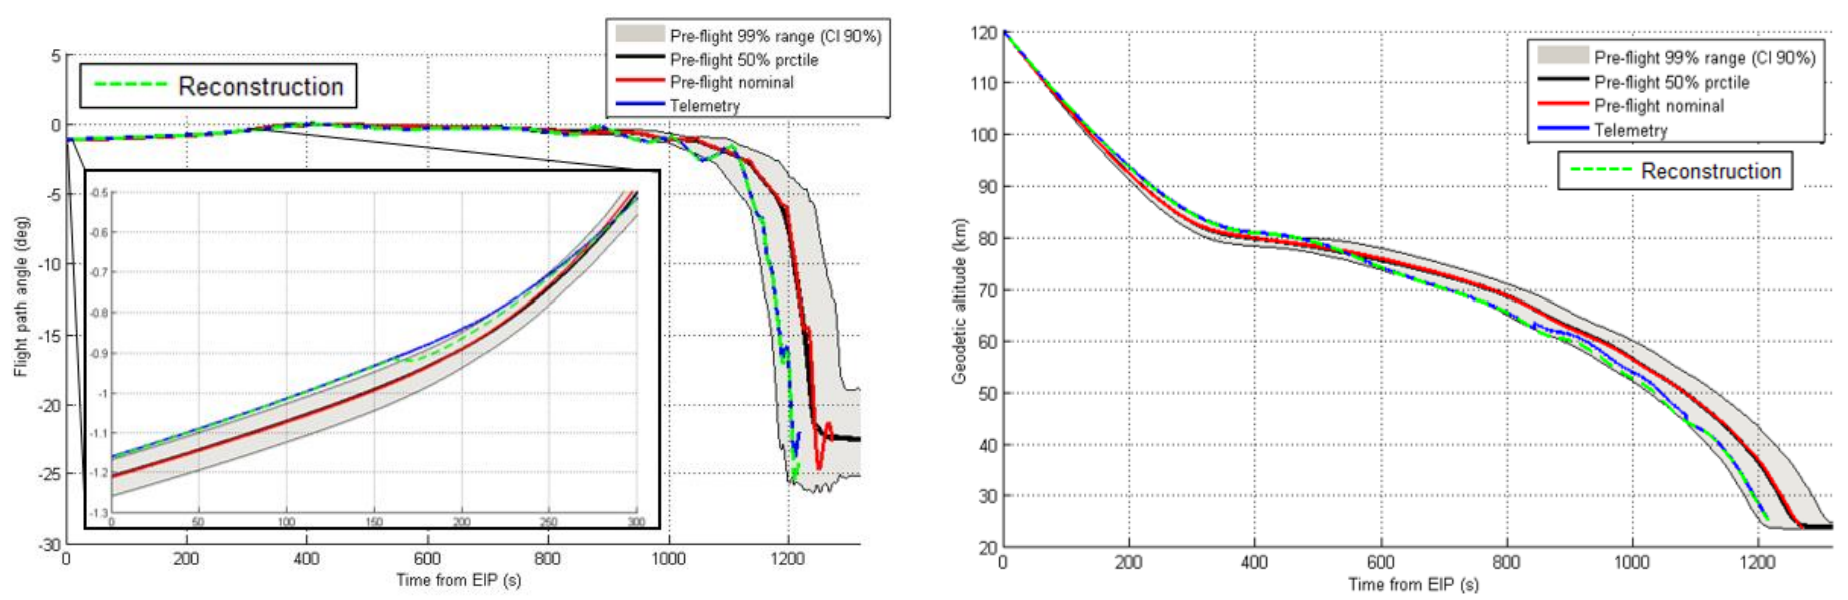
\includegraphics[width=1\linewidth]{descent_altitude.png}
\caption{IXV reentry descent angle (left) and altitude(right) profiles \cite{bonetti2019ixv}}
\label{descent_altitude}
\end{figure}

As seen in the left plot of Figure~\ref{descent_altitude}, the descent angle is nearly zero within the time range of 300~s to 900~s, during which the decrease in altitude is shallow, as seen in the right plot of the figure. For comparison, the altitude profile for two descent angles is shown in Figure~\ref{suave_altitude_profile}.

\begin{figure}[ht]
\centering
\begin{subfigure}[b]{0.49\textwidth}
\centering
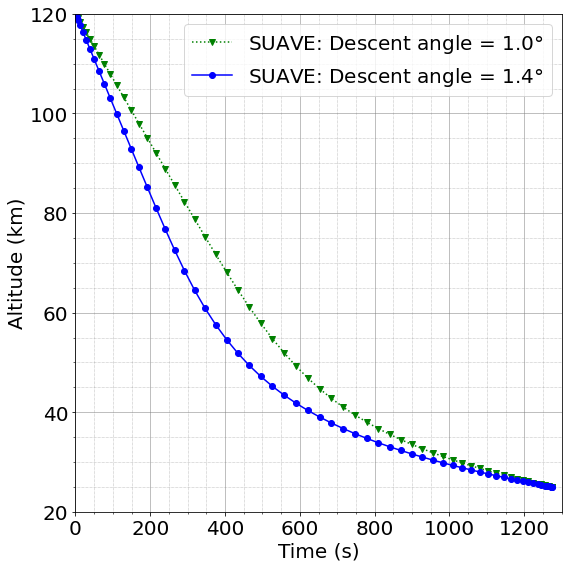
\includegraphics[width=\textwidth]{IXV_altitude_history_1976.png}
\caption{Predicted altitude history}
\label{suave_altitude_profile}
\end{subfigure}
~
\begin{subfigure}[b]{0.49\textwidth}
\centering
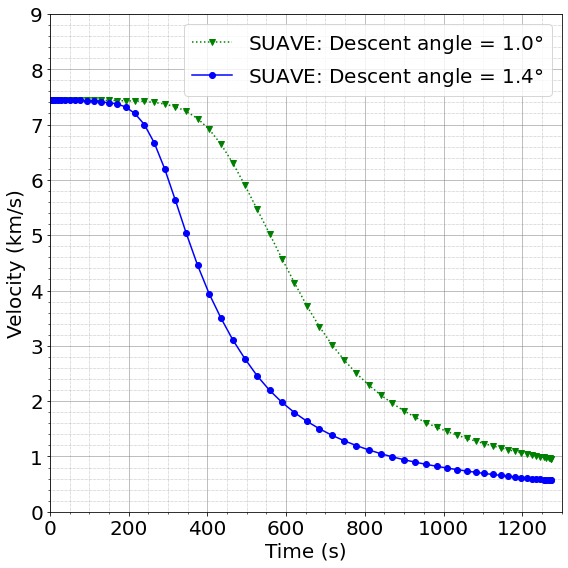
\includegraphics[width=\textwidth]{IXV_velocity_history_1976.png}
\caption{Predicted veloctiy history}
\label{suave_velocity_profile}
\end{subfigure}
\caption{Comparison of SUAVE predicted altitude and velocity history for two descent angles}
\end{figure}

Compared to the actual altitude profile shown in the right plot of Figure~\ref{descent_altitude}, it is evident that a constant descent angle considered in the SUAVE model contributes to an inaccurate prediction of the altitude profiles plotted in Figure~\ref{suave_altitude_profile}. Due to the correlation between atmospheric density and the reentry velocity profile (Equation~\eqref{equ_glide}), an incorrect altitude would lead to incorrect velocity profile, shown in Figure~\ref{suave_velocity_profile}, and in turn causing inaccurate predictions of the vehicle deceleration profile, seen in Figure~\ref{valid2_2}. These inaccuracies can be corrected in SUAVE using a detailed description of the reentry trajectory with piecewise input of descent angle in each trajectory segment.

\subsubsection{Aerothermal results}
First, using the aerothermal formulations developed in the present work, the shock structure is computed at 374~s at which Mach 15 is achieved in the simulation of the IXV reentry mission. The computed 2D and 3D shock structure is plotted in Figure~\ref{SUAVE_shock} and is compared with numerical and experimental results at Mach 15 as shown in Figure~\ref{valid_shock} \cite{paris2011experimental}.

\begin{figure}[h!]
\centering
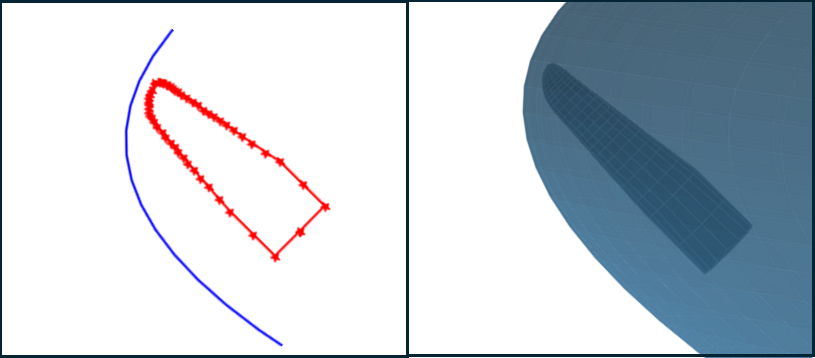
\includegraphics[width=0.6\linewidth]{IXV_shock_plot.png}
\caption{2D and 3D shock structure around IXV at angle of attack of 45$\degree$}
\label{SUAVE_shock}
\end{figure}

\begin{figure}[h!]
\centering
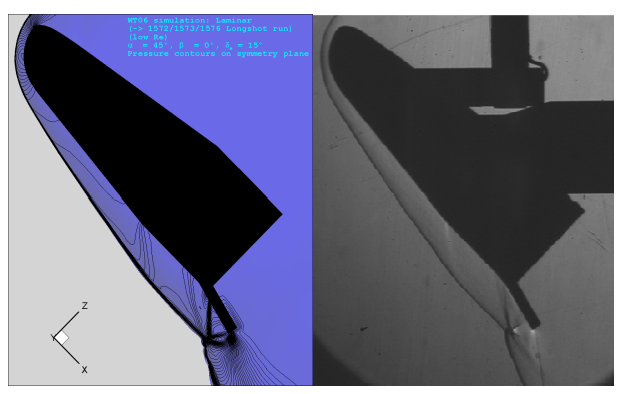
\includegraphics[width=0.6\linewidth]{shock_validation.png}
\caption{Numerical (left) and experimental (right) shock structure around IXV test model at angle of attack of 45$\degree$ \cite{paris2011experimental}}
\label{valid_shock}
\end{figure}
It can be seen from Figures~\ref{SUAVE_shock} and ~\ref{valid_shock} that predicted shock standoff distance is closely matched, however, that over the windside surface of IXV is larger than the experimental and numerical observation of IXV test model. This could be attributed to the scaling down of IXV for testing and computing purposes, which leads to reduced stagnation radius and consequently reduced shock stand off distance. Here, it is promising that low-fidelity formulations are capable of approximating the shock structure over the reentry geometry, which reduces the cost of computing significant post shock results.

Secondly, the temporal stagnation heat flux during the IXV reentry mission is estimated and plotted in Figures~\ref{valid3_1} and \ref{valid3_2}.
\begin{figure}[ht]
\centering
\begin{subfigure}[b]{0.49\textwidth}
\centering
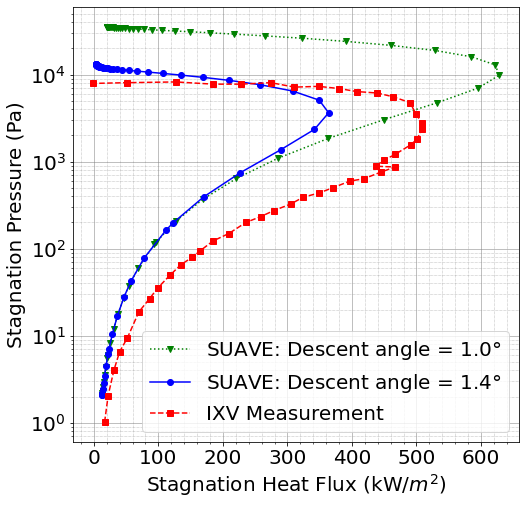
\includegraphics[width=\textwidth]{IXV_heat_flux_pressure_1976.png}
\caption{Heat flux vs pressure at stagnation point}
\label{valid3_1}
\end{subfigure}
~
\begin{subfigure}[b]{0.49\textwidth}
\centering
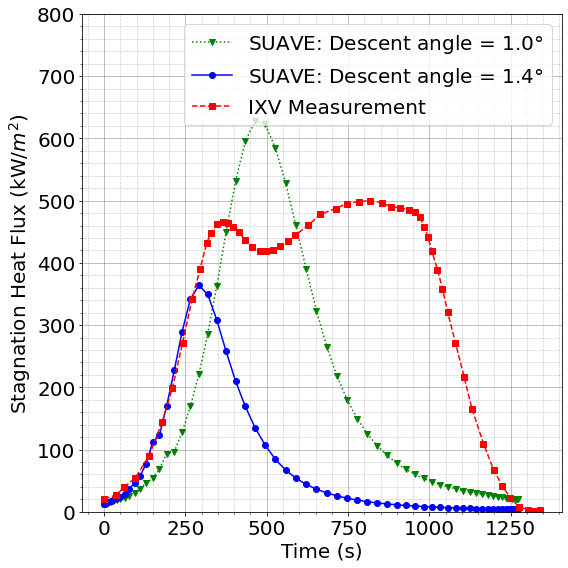
\includegraphics[width=\textwidth]{IXV_heat_flux_history_1976.png}
\caption{Heat flux history at stagnation point}
\label{valid3_2}
\end{subfigure}
\caption{Comparison SUAVE simulated IXV stagnation point heat flux and pressure at different descent angles vs IXV measurement}
\end{figure}
It is evident from Figure~\ref{valid3_1} that both simulations with different descent angles show a significant deviation from the measured data of heat flux versus pressure at the stagnation point. However, during the initial phase of reentry, the simulated time-history of stagnation heat flux, shown in Figure~\ref{valid3_2}, matches well with IXV measurement for a descent angle of 1.4$\degree$. Thus, the mismatch in the simulated values for the descent angle 1.4$\degree$ from Figure~\ref{valid3_1} is due to the mismatch in the stagnation pressure during the initial reentry phase. Since stagnation pressure is a strong function of freestream conditions, this trend can be attributed to inaccuracies in freestream properties, owing to the altitude mismatch caused by constant descent angle input, as discussed in detail in the previous section. The inaccuracies in stagnation pressure are then applicable to simulations with descent angle 1.0$\degree$ as well, leading to its mismatch in both stagnation pressure and heat flux, as seen in Figures~\ref{valid3_1} and \ref{valid3_2}.
Although the predicted heat flux from the case with descent angle 1.4$\degree$ follows the measurement closely during the initial stages of reentry, the prediction deviates after 250~s after reaching a peak value of 350~kW/m$^{2}$. This mismatch is also attributed to the descent angle input method. Since the IXV flight descent angle is nearly zero between 300~s to 900~s (left plot of Figure~\ref{descent_altitude}), the altitude does not decrease significantly during this time range, leading to the formation of a steady peak value of the measured heat flux in Figure~\ref{valid3_2}. This observation is also evident from Figure~\ref{valid3_2}, where a lower descent angle of 1.0$\degree$ leads to higher peak stagnation point heat flux values. Thus, a series of reducing descent angles, as seen in the initial phase of the IXV flight (left plot of Figure~\ref{descent_altitude}), can lead to an increase in peak heat flux than that simulated with descent angle 1.4$\degree$. However, it should be noted that, if the simulations were carried out with measured descent angle profile, the simulated heat flux peak will be higher than the measured values (peak heat flux at the descent angle 1.0$\degree$ surpassed the measured peak).

%The heat flux profile for descent angle of 1.4$\degree$ in Figure~\ref{valid3_2} shows a good match with measured data during the initial phase of  general mismatch in predicted heat flux at a good overall match, however, the peak heat flux is overpredicted by the present formulations. Significant deviations from measured data are observed as the IXV mission progresses, demonstrating the need for more physics-based models (shock-structure and near-wall modeling for shock-induced heating). %This shows that standard reentry heat flux correlations, similar to equation~\ref{heat_flux}, are suited to rarefied atmosphere, whereas near-wall models and conjugate heat transfer formulations are key to acurately predicting peak and integral heat flux profiles in denser atmosphere.

Next, stagnation point surface temperature history is calculated using the estimated heat flux profile for descent angle 1.4$\degree$.  Both the trends are plotted in Figure~\ref{surf_therm}. The thermophysical properties and thickness of the IXV nose material, Zircar, are taken from the reported literature \cite{Massimo2008}. At reentry point, the temperature throughout the material is assumed to be at 300K and the inner wall of the material is considered to be at 300K throughout the mission.

\begin{figure}[h!]
\centering
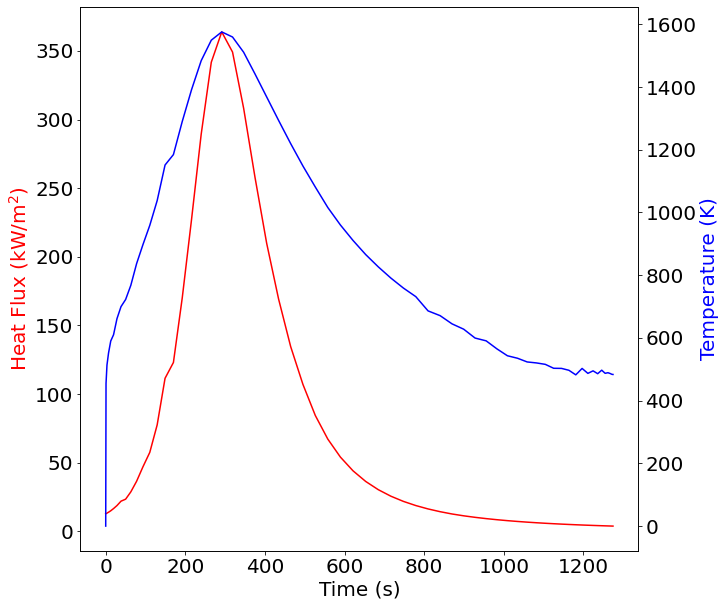
\includegraphics[width=0.7\linewidth]{IXV_stag_thermal.png}
\caption{SUAVE predicted stagnation point surface heat flux and temperature histories for descent angle of 1.4$\degree$}
\label{surf_therm}
\end{figure}
It can be seen from Figure~\ref{surf_therm} that the transience in surface temperature due to integral heat load at stagnation point is captured by the simulation. Initial rise in temperature is noted, which is attributed to the non-zero initial heat flux at start of reentry. For a peak heat flux of 350kW/m$^{2}$, the peak stagnation point temperature is simulated to be 1580K which is higher than the measured value of 1350K \cite{buffenoir2017ixv}. This trend is similar to that observed for Apollo simulations in Section 3.2. However, as opposed to the large difference in prediction and measurement in Apollo case (4000K predicted against 2200K measured), that difference in IXV is lesser. This can be attributed to reduced effects of ionization and surface ablation, due to lower overall surface temperatures. However, it should be kept in mind that the IXV flight peak heat flux is higher than the peak heat flux in Figure~\ref{surf_therm} and also that the simulated heat flux can be much higher than the measured peak (Figure~\ref{valid3_2}), making the present simulated peak temperature a conservative value.

Finally, the predicted aerothermal and trajectory performance parameters of the IXV mission are plotted against altitude in Figure~\ref{res1}. It is important to note that the peak aerothermal heat flux does not necessarily correspond to the point of maximum deceleration or Mach number. This information is critical in determining the focus conditions for high-fidelity models and in designing parameters for an active thermal protection system. 

\begin{figure}[ht]
\centering
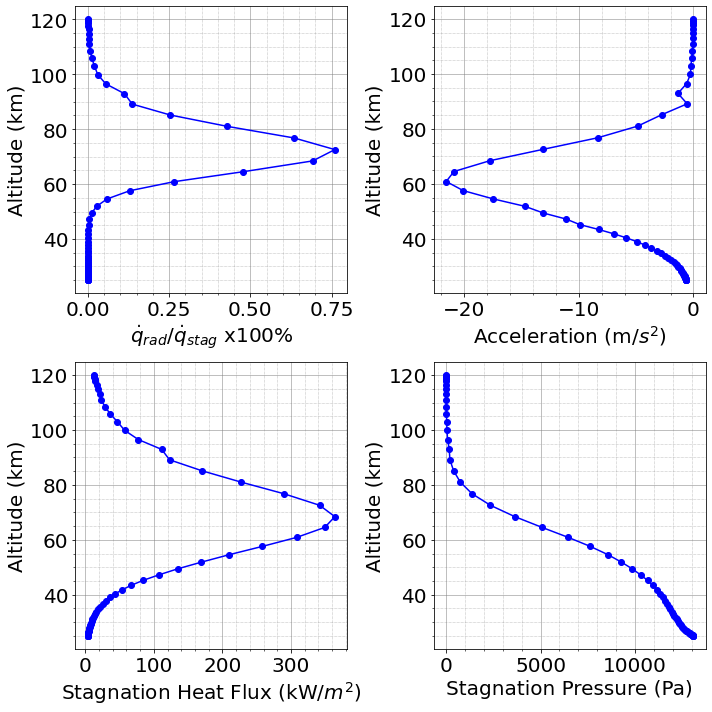
\includegraphics[width=0.6\linewidth]{IXV_performance_vs_altitude_1976.png}
\caption{SUAVE predictions of IXV mission performance vs altitude}
\label{res1}
\end{figure}

It is also evident from Figure~\ref{res1} that radiative heat flux is negligible during IXV reentry. This is expected since radiation effects have been reported to be insignificant for reentry speeds lower than 9000~m/s \citep{brandis_benchmark_2017,winter_radiation_2019}. %For instance, reentry of the Hayabusa capsule at 11700~m/s resulted in radiation heat flux contribution of 18\% towards stagnation point heat flux \citep{winter_radiation_2019}. However, experimental studies by \cite{brandis_benchmark_2017} showed that the radiation effects drop by an order of magnitude as reentry velocity is 9000~m/s.

\section{Discussion and Conclusion}

%\rw{summarise limitations of current work / models, discuss next steps}

The estimation of the maximum aerothermal loading is a critical design parameter for hypersonic and reentry vehicles. The maximum thermal loading will dictate the material, structure, and thermal protection system of a hypersonic vehicle. It is therefore of interest to predict the time-varying conditions at peak thermal load and optimize trajectory and operational characteristics to align with other design constraints. We present the development of an integrated, low-fidelity aerothermal predictive framework based on SUAVE. The framework uses low-fidelity models for a computationally efficient estimation of the thermal loading by: (1) estimating the stagnation point heat flux; (2) approximating the shock structure around the vehicle; and (3) calculating the distributed heat load. These thermal estimates can then be used to estimate the conjugate heat transfer conditions in the vehicle.

Ultimately, this framework can help estimate critical thermal operating points during a hypersonic reentry mission, which can be studied in more depth using high-fidelity computational fluid dynamics, typically RANS or LES. There are a number of limitations to using a low-fidelity framework, with most estimations based on empirical models that may not generalize to every operating condition. For example, the total heat flux is heavily dependent on the estimation of the transition location, which in turn, is a highly sensitive parameter to angle of attack, roughness, crossflow, etc. Similarly, many models rely on geometrical simplifications (e.g. conjugate heat transfer modeling or shock structure estimation), which may not account for important geometrical and flow features, such as shock-shock interactions and compression corners. Despite these approximations, these low-order models allow for a computationally tractable and robust optimization of the trajectory and operational characteristics, which is the ultimate objective of this work. Future work will focus on higher-fidelity modeling of the identified critical states during reentry.

%\input{latex-template-whitepaper-basic-master/originalSubmission}

\begin{acknowledgments}
This work stems from a NATO Unclassified report contribution that was submitted as part of the NATO-STO-AVT-SET 396 Resesarch Symposium in Koblenz, Germany in October 2024. 
\end{acknowledgments}

\appendix 
\section*{A.0 APPENDIX}
\subsection*{A.1 \quad Orion Experiments Additional Validation Cases}

\begin{table}[ht]
\caption{Additional validation test conditions from \cite{hollis_aeroheating_2009}}
\label{hollis_more_inputs}
\begin{center}
\begin{tabular}{c c c c c c c c}
\textbf{$AoA (deg)$} &  \textbf{$V_\infty(\frac{m}{s})$} & \textbf{$\rho_\infty (\frac{kg}{m^{3}})$} & \textbf{$P_\infty (Pa)$} & \textbf{$M_\infty$} & \textbf{$T_{wall} (K)$} & \textbf{$H_0 - H_{300K} (\frac{J}{kg})$} & \textbf{$Re_\infty (\frac{1}{m})$}\\ 
\hline \\
24 & 1287 & 0.105 & 2240 & 7.45 & 318  & 5.91e5 & 2.7e7\\
24 & 1403 & 0.224 & 5490 & 7.57 & 376  & 7.59e5 & 5.5e7\\
24 & 1347 & 0.382 & 8150 & 7.79 & 369  & 6.70e5 & 10e7\\
24 & 1468 & 0.110 & 1600 & 10.3 & 321  & 8.51e5 & 4.8e7\\
24 & 1455 & 0.148 & 2030 & 10.4 & 326  & 8.01e5 & 6.5e7\\
\hline\\
32 & 1312 & 0.105 & 2310 & 7.45 & 322 & 6.20e5 & 2.7e7 \\
32 & 1419 & 0.225 & 5640 & 7.57 & 393 & 7.83e5 & 5.5e7 \\
32 & 1380 & 0.376 & 8400 & 7.80 & 394 & 7.19e5 & 10e7 \\
32 & 1480 & 0.110 & 1610 & 10.3 & 331 & 8.34e5 & 4.8e7 \\
32 & 1478 & 0.148 & 2120 & 10.4 & 336 & 8.31e5 & 6.5e7 \\
% \hline
\end{tabular}
\end{center}
\end{table}

\begin{figure}[h!]
\centering
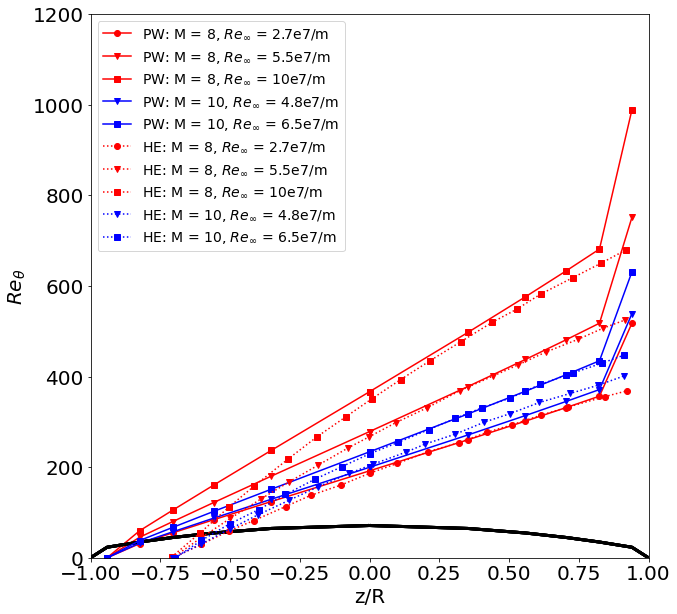
\includegraphics[width=0.7\linewidth]{Re-24-hollis.png}
\caption{$Re_\theta$ vs normalized capsule height at angle of attack = 24$\degree$. HE: Hollis et al Experiment, PW: Present Work.}
\label{Re-24-hollis}
\end{figure}

\begin{figure}[h!]
\centering
\begin{subfigure}[b]{0.49\textwidth}
\centering
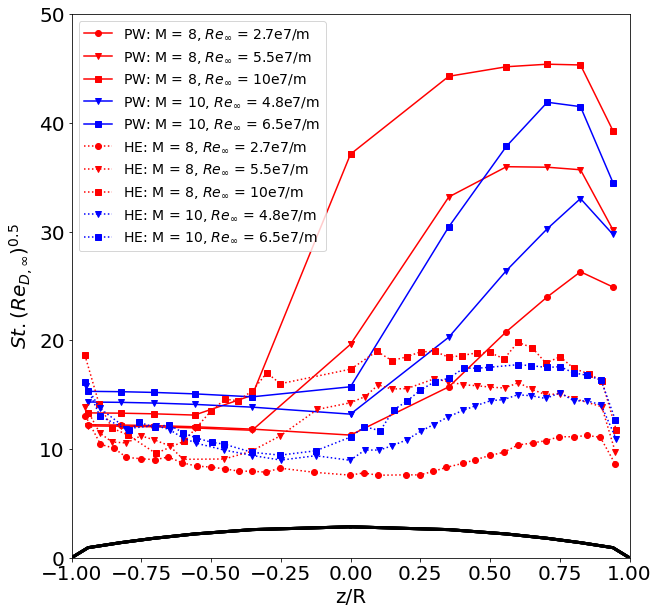
\includegraphics[width=\textwidth]{St-24-hollis.png}
\caption{Original correlation of \cite{hollis_aeroheating_2009}}
\label{St-24-hollis}
\end{subfigure}
~
\begin{subfigure}[b]{0.49\textwidth}
\centering
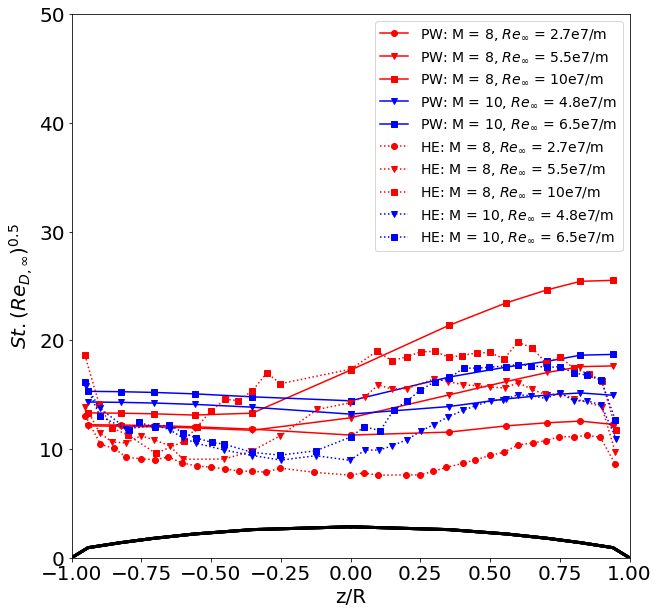
\includegraphics[width=\textwidth]{St-24-hollis-new.png}
\caption{Modified correlation}
\label{St-24-hollis-new}
\end{subfigure}
\caption{Normalized heat flux vs normalized capsule height at 24$\degree$ angle of attack. HE: Hollis et al Experiment, PW: Present Work}
\end{figure}

\begin{figure}[h]
\centering
\begin{subfigure}[b]{0.49\textwidth}
\centering
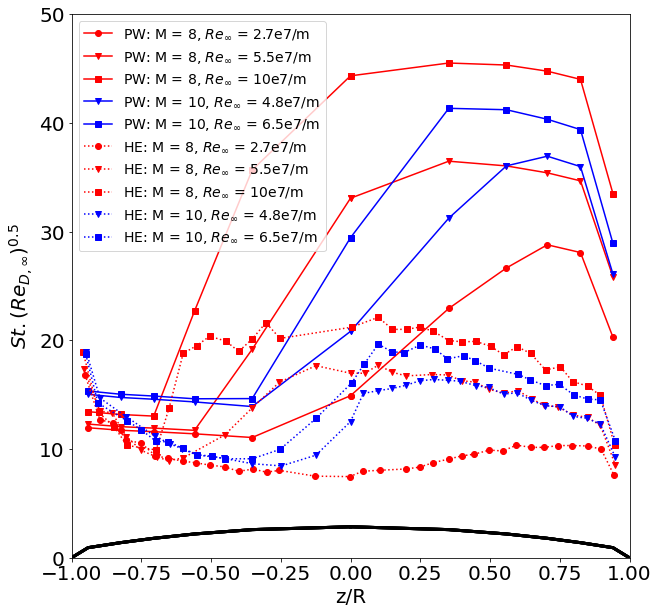
\includegraphics[width=\textwidth]{St-32-hollis.png}
\caption{Original correlation of \cite{hollis_aeroheating_2009}}
\label{St-32-hollis}
\end{subfigure}
~
\begin{subfigure}[b]{0.49\textwidth}
\centering
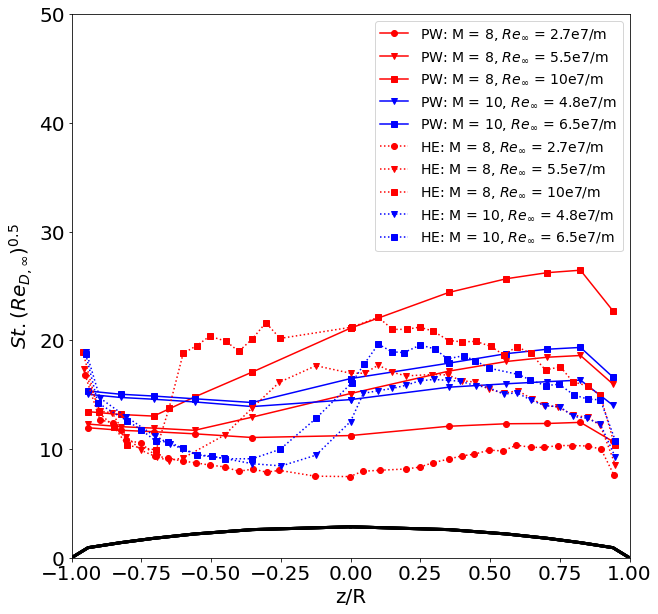
\includegraphics[width=\textwidth]{St-32-hollis-new.png}
\caption{Modified correlation}
\label{St-32-hollis-new}
\end{subfigure}
\caption{Normalized heat flux vs normalized capsule height at 32$\degree$ angle of attack. HE: Hollis et al Experiment, PW: Present Work}
\end{figure}

% ===================================%
%%%%%%%%% Bibliography %%%%%%%%%
% ===================================%



\clearpage
\bibliography{references}


\end{document}
%
% ****** End of file aipsamp.tex ******